%broadband performance measurements


\documentclass{sig-alternate-10pt}
%\documentclass{IEEEtran}
\usepackage{boxedminipage}
\usepackage{verbatim}

%\usepackage[numbers]{natbib}

\usepackage{url}
\usepackage{balance}
\usepackage[colorlinks=true,linkcolor=black,urlcolor=black,citecolor=black]{hyperref}
\usepackage{breakurl} % after hyperref ¿and url?

\usepackage[dvipsnames,usenames,table]{xcolor}

%\usepackage{eso-pic}
\usepackage{graphicx}

%\usepackage{subfig}
\usepackage{caption}
\usepackage{subcaption}

%\usepackage{subfigure}

\usepackage{pseudocode}

%%%%%%%%%%% comments, notes, etc. from here ...
\newcommand{\tr}[1]{\textcolor{Red}{#1}}
\newcommand{\tg}[1]{\textcolor{Green}{#1}}
\newcommand{\tb}[1]{\textcolor{Blue}{#1}}
%\newcommand\rem[1]{}
\newcommand{\rem}[1]{\textcolor{Red}{#1}}%
\newcommand{\timeofwriting}{ (April 2014) }

%\renewenvironment{comment}{}{}

\usepackage{comment}

\specialcomment{notecommenti}%
	{\begingroup\color{Red}}%
	{\endgroup}
%\excludecomment{notecommenti}
%\includecomment{notecommenti}

\specialcomment{segnapostoSiToglie}%
	{\begingroup\color{Blue}}%
	{\endgroup}

%% selectively disable comments:
\excludecomment{notecommenti}
\excludecomment{robaTolta}
\renewcommand\rem[1]{}
%\excludecomment{segnapostoSiToglie}

%%%%%%%%%%% comments, notes, etc. end here.

\begin{document}

\begin{notecommenti}
\subsubsection{TO DO}
\begin{itemize}
\item clean from clutter
\item add intro
\item add SoA
\item add substitutes for cut parts
\item compare with Gill
\end{itemize}
\end{notecommenti}


\title{Measuring Broadband Performance for Home Users in Pakistan using BISmark\titlenote{This study has been carried out with help of Project BISmark (Broadband Internet Service Benchmarking).}
\\}
%Format\titlenote{(Does NOT produce the permission block, copyright information nor page numbering). For use with ACM\_PROC\_ARTICLE-SP.CLS. Supported by ACM.}}
%\subtitle{[Extended Abstract]
%\titlenote{A full version of this paper is available as
%\textit{Author's Guide to Preparing ACM SIG Proceedings Using
%\LaTeX$2_\epsilon$\ and BibTeX} at
%\texttt{www.acm.org/eaddress.htm}}}
%
% You need the command \numberofauthors to handle the 'placement
% and alignment' of the authors beneath the title.
%
% For aesthetic reasons, we recommend 'three authors at a time'
% i.e. three 'name/affiliation blocks' be placed beneath the title.
%
% NOTE: You are NOT restricted in how many 'rows' of
% "name/affiliations" may appear. We just ask that you restrict
% the number of 'columns' to three.
%
% Because of the available 'opening page real-estate'
% we ask you to refrain from putting more than six authors
% (two rows with three columns) beneath the article title.
% More than six makes the first-page appear very cluttered indeed.
%
% Use the \alignauthor commands to handle the names
% and affiliations for an 'aesthetic maximum' of six authors.
% Add names, affiliations, addresses for
% the seventh etc. author(s) as the argument for the
% \additionalauthors command.
% These 'additional authors' will be output/set for you
% without further effort on your part as the last section in
% the body of your article BEFORE References or any Appendices.

\numberofauthors{1} %  in this sample file, there are a *total*
% of EIGHT authors. SIX appear on the 'first-page' (for formatting
% reasons) and the remaining two appear in the \additionalauthors section.
%
\author{
% You can go ahead and credit any number of authors here,
% e.g. one 'row of three' or two rows (consisting of one row of three
% and a second row of one, two or three).
%
% The command \alignauthor (no curly braces needed) should
% precede each author name, affiliation/snail-mail address and
% e-mail address. Additionally, tag each line of
% affiliation/address with \affaddr, and tag the
% e-mail address with \email.
%
% 1st. author
%\alignauthor
%Muhammad Faheem Awan, Saad Qaisar \\ %\titlenote{Dr.~Trovato insisted his name be first.}\\
%       \affaddr{School of Electrical Engineering and Computer Science, NUST}\\
      % \affaddr{}\\
 %      \affaddr{Islamabad, Pakistan}\\
  %     \email{(10mscsemawan,saad.qaisar)@seecs.edu.pk}
% 2nd. author
%\alignauthor
%Saad Qaisar \\%\titlenote{The secretary disavows
%any knowledge of this author's actions.}\\
 %     \affaddr{School of Electrical Engineering and Computer Science,NUST}\\
       %\affaddr{}\\
  %     \affaddr{Islamabad, Pakistan}\\
   %    \email{saad.qaisar@seecs.edu.pk}
% 3rd. author
%\alignauthor Lars Th{\o}rv{\"a}ld\titlenote{This author is the
%one who did all the really hard work.}\\
%       \affaddr{The Th{\o}rv{\"a}ld Group}\\
 %      \affaddr{1 Th{\o}rv{\"a}ld Circle}\\
 %      \affaddr{Hekla, Iceland}\\
  %     \email{larst@affiliation.org}
%\and  % use '\and' if you need 'another row' of author names
% 4th. author
%\alignauthor Lawrence P. Leipuner\\
 %      \affaddr{Brookhaven Laboratories}\\
  %     \affaddr{Brookhaven National Lab}\\
   %    \affaddr{P.O. Box 5000}\\
    %   \email{lleipuner@researchlabs.org}
% 5th. author
%\alignauthor Sean Fogarty\\
 %      \affaddr{NASA Ames Research Center}\\
  %     \affaddr{Moffett Field}\\
   %    \affaddr{California 94035}\\
    %   \email{fogartys@amesres.org}
% 6th. author
%\alignauthor Charles Palmer\\
 %      \affaddr{Palmer Research Laboratories}\\
  %     \affaddr{8600 Datapoint Drive}\\
   %    \affaddr{San Antonio, Texas 78229}\\
    %   \email{cpalmer@prl.com}
}
% There's nothing stopping you putting the seventh, eighth, etc.
% author on the opening page (as the 'third row') but we ask,
% for aesthetic reasons that you place these 'additional authors'
% in the \additional authors block, viz.
%\additionalauthors{Additional authors: John Smith (The Th{\o}rv{\"a}ld Group,
%email: {\texttt{jsmith@affiliation.org}}) and Julius P.~Kumquat
%(The Kumquat Consortium, email: {\texttt{jpkumquat@consortium.net}}).}
%\date{30 July 1999}
% Just remember to make sure that the TOTAL number of authors
% is the number that will appear on the first page PLUS the
% number that will appear in the \additionalauthors section.


\maketitle
\begin{sloppypar}
\begin{abstract}
Even though broadband Internet enjoys wide penetration in Pakistan, performance of fixed and wireless broadband has not been thoroughly investigated upon from an end user's perspective. To the best of our knowledge, no independent study exists to date documenting home user broadband experience in Pakistan. This dearth of evidence is noteworthy since regularly observing and checking broadband performance is fundamentally important both for consumer and regulatory consumption, most importantly to keep a check if users are getting services they are paying for and regulators can make conversant decisions. To address this gap, we conducted a pilot study of both fixed and wireless broadband connections in Pakistan through deployment of programmable wireless routers for home users in collaboration with Project BISmark, Georgia Tech, Atlanta, USA. This paper presents the methodology and results of measurement based analysis of logs collected using BISmark routers. Surprisingly, our findings are in line with findings in  ~\cite{26} suggesting that consumers in Pakistan are not getting advertised speeds, wireless broadband leaves behind fixed broadband in areas where both are available, and speed is not the only limiting factor on performance. Our results show that monitoring broadband performance provides enough information for consumers and policy-makers alike. Finally, limiting factors such as latency mean that investing in local server infrastructure will also go a long way in refining broadband experience for Pakistani users. This study is an extension of work previously performed at South Africa using BISmark. Our contribution to information and communication technologies community (IC\&T) includes first systematic study of broadband performance in Pakistan that can serve as an example for monitoring broadband performance in similar developing countries.
\end{abstract}

% A category with the (minimum) three required fields
\category{C.2.3}{Computer-Communication Networks}{Network Operations-Network Management}
%A category including the fourth, optional field follows...
\category{K.4.1}{Computers and Society}{Public Policy Issues}[regulation, performance measures]

\terms{Performance, Measurement, Management }

\keywords{Broadband performance, quality of service, consumer protection, internet benchmarking} % NOT required for Proceedings

\section{Introduction}
\indent Since wide-spread adoption of Internet, a community of researchers has focused their efforts to improve and evolve the technology. A significant amount of research is dedicated to improve access network quality for an end-user. In Pakistan, broadband service adoption is on a fast lane. All major service providers (ISPs) are advertising new data packages at increasingly lower cost in order to capture market. Despite increase in broadband penetration in Pakistan, very little knowledge exists about country's broadband performance. Broadband users and authorities do not have access to systematic assessments particularly from a home user's perspective. This dearth of substantiation is troublesome, aside from cost ~\cite{chetty:cap}, if performance is not up to mark, it affects usage of broadband ~\cite{10,25}  resulting in decline of country's development indicators ~\cite {24}. In order to discourse this space between authorities, users and broadband providers, a need for measuring broadband performance arises in Pakistan in order to ensure that ISPs fulfill their promise of advertised rates, users use reliable connection and officials can undertake informed decisions ~\cite{12,15,16}. Hitherto, to the best of our knowledge, no methodological independent study of fixed broadband land line/wireless Internet performance has been steered in Pakistan for home users. This manuscript aims to address this gap as a first step, facilitating users, broadband providers and regulators towards improvement of Internet infrastructure. Our main objective is collecting realistic evidence about quality of broadband connectivity in Pakistan.

\indent The following questions were under observation.
\begin{itemize}
  \item Are home users getting what their Internet service provider (ISP) is advertising to offer them?
  \item Are users attaining steady performance?
  \item What are other factors except throughput that affect broadband performance?
\end{itemize}
\indent In order to answer these questions, in the first phase, we deployed custom home network routers at 15 different testing sites in Northern region of Pakistan, incities of Islamabad (capital city), Rawalpindi, Abbottabad and Wah. Islamabad and Rawalpindi are considered as privileged localities with high-end users having set-up of almost all major ISPs located within the city or premises. On the contrary, Wah and Abbottabad represent lesser developed urban settings. The routers are given to users having different ISPs and service plans helping gather throughput and latency measurements over a period of 4 months from last quarter of 2013 to early 2014 with approximately 10 measurements on daily basis. \\
\indent Through the course of our study, we gained some fundamental insights which may be interesting both to end-users and research community. First of all, majority of customers are not getting the service which they are paying for i.e. they are not achieving throughput rates that are advertised to them by their service providers. These results so attained controvert to results of studies conducted similarly in developed countries such as United Kingdom \& United States ~\cite{16} and are in line with a recent study in developing world by Feamster et al ~\cite{26}.In case of Feamster et al, comparison is made in between mobile broadband ISP’s and land line ISP’s whereas in Pakistan comparison is made between fixed wireless broadband ISP’s and land line ISP’s. Regions where both landline and wireless (fixed) operate, wireless (fixed) outperforms landline. This explains the exponential growth in number of consumers using fixed wireless broadband ~\cite{28}. Third, and conceivably utmost significant, throughput that an ISP offers is only part of story, equally important is latency to web-sites and services that users actually visit. Physical distance of users from servers of most popular websites like Facebook, Twitter etc. generates latency values in several hundreds of milliseconds resulting in unreliable performance of an ISP. . For servers which are physically far away but have profound routes, results in low values of latency. \\
\indent Our findings infer that benchmarking ISP performance in a country enlightens both customers and regulators. Regulators and policy makers can provide favorable environment so that companies invest in creating local servers or servers nearby for popular websites like Facebook in order to reduce latency values which in turn enriches user experience.\\
\indent Rest of the paper is structured as follows.  First of all, we discuss motivations and background of our study. We present metrics and methods used for measuring broadband performance. We sketch advantages of our approach for measuring broadband performance compared with alternative approaches. We describe challenges faced during period of measurements typical in developing countries. We present our method and results of our ongoing study aiming to benchmark ISPs (land line and wireless (fixed)) across Pakistan.  Finally, we provide recommendations for improvement in prevailing conditions and conclusion.

\section{BACKGROUND}
In this section, we present background work regarding broadband performance measurements in Pakistan along with inspiration for measuring broadband performance.
\subsection {Broadband in Pakistan}
Pakistan is on fast lane in terms of broadband Internet. In Pakistan, there are nearly 30 million Internet users with penetration rate of 16\% ~\cite{01}. There are almost 50 Internet service providers ~\cite{01} where number of customers using broadband is nearly 2.2 Million ~\cite{02}. Pakistan Internet user's growth rate is 2nd highest in SAARC countries in accordance with its population ~\cite{02}. Broadband in Pakistan includes fixed line via Digital Subscriber line (DSL), Fiber to the Home (FTTH), 3G USB modem and WiMax (IEEE802.16d) connections.

\indent Pakistan is less progressive in terms of regulating in spite of greater Internet penetration rate. In Pakistan,  broadband policy was drafted in December 2004 ~\cite{03}. After 2004, number of ISPs came into existence and broadband shot in popularity. Even though policy exists since 2004, there are no significant updates on policies that were drafted in 2004. For instance, the policy draft does not address how quality of broadband is monitored and regulated. Our study will help authorities in order to draft new policies for continuous monitoring and regulation of broadband ISPs.

\subsection {Existing Measurements in Pakistan}
There is scant data available regarding broadband performance in Pakistan from a home user's perspective. For instance, the RIPE Atlas project  ~\cite{21} uses custom probes for analyzing Internet measurements though in Pakistan, only 2 probes are registered with the project for measurements. Similarly, host based measurements for different countries including Pakistan are available from OOKLA ~\cite{20} and Akamai ~\cite{05}. According to OOKLA Net index, Pakistan falls on 174th position with average download speeds of 2.3 Mbps and falls on 170th position with average upload speed of 1 Mbps ~\cite{07}. Akamai (Q4 2013 report) ~\cite{05} reports average connection speed of 1.4Mbps and broadband adaptation rate of 1.2 percent in Pakistan ~\cite{28}.\\
\indent Regardless of OOKLA and AKAMAI statistics having thousands of record points, they do not provide in depth analysis of broadband performance in a specific country regarding: user's broadband service provider, user's service plan, variation in performance over time and performance issues. Our study may have less data points than OOKLA and AKAMAI given the cost and number of tools available, it gives more insight on home user's experience since router based approach takes measurements from inside a home over time and gives a clearer picture of both land line and fixed wireless broadband performance.

\subsection {Need for measuring broadband Performance in Pakistan}
Increasing broadband penetration in Pakistan necessitates independent benchmarking of ISPs in order to improve home networks. Measuring broadband performance is also significantly important for auditing and accountability of ISPs. Measuring broadband performance will help in order to fulfill gap between planned and achieved rates. This will help authorities in terms of regulating ISPs. Measuring broadband can also facilitate service providers in terms of investment, where they can invest in order to improve the network.


\section {Methodology}
The focal drive of this paper is to benchmark the internet service providers in Pakistan directly from the user’s home gateway. In this section, we describe the methodology of our study. We also discuss metrics and methods typically used for measuring broadband performance along with datasets available. We describe tools we implemented for measuring broadband performance and how we recruit users for this study. At the end of this section, we list down challenges we experienced and how we counterpart these challenges.

\subsection {Measurement metrics \& Approaches}
We define metrics and approaches used for computing broadband performance.
\subsubsection {Performance Metrics}
Most widely used metrics for measuring broadband performance include download and upload throughput, latency, jitter and packet loss. Upload and download throughput are generally referred as upstream and downstream throughput ~\cite{08,12,16}.\\
\indent Download speeds are a measure of Internet traffic towards the user from local or international servers and is measured in Megabits per second (Mbps). Slow download speeds affect file downloading, streaming videos and other online applications that require high download speeds.\\
\indent Upload speeds measure the transfer of Internet traffic from user towards local or international servers and is measured in Mbps. Upload speeds affect real-time interactive applications like video conferencing, voice chat, online gaming etc.\\
\indent Latency is the measure of round trip time taken by a packet from source to destination and back, measured in milliseconds (ms). Latency mostly distresses real time applications such as VOIP and online gaming. Online gaming is intolerably affected by high latency values.\\
\indent Jitter is the measure of un-evenness in latency measurements. High jitter affects real time applications such as gaming, video conferencing, and VOIP services.\\
\indent Packet loss is number of packets that fail to touch the destination either resulting from upstream or downstream. Packet loss is measured in percentage of loss. High percentages of packet loss degrade performance of broadband connection.\\
\indent Upload and download speeds are measured by sending a file from source to destination and calculating time to reach the destination. Similarly, latency measurements are taken by using PING and FPING tests. PING and FPING are network functions that send file to the destination and wait for a response. Jitter has been calculated using measure for change in latency. These are most viable and accepted methods and metrics used for measuring broadband performance ~\cite{23}.
\subsection {Measurement Approaches}
Number of methods and techniques are used in order to measure broadband performance. One method is taking measurements from the end host. Such types of measurements are called host-based measurements. They are mostly called active measurements since they involve continuously sending or receiving data on the user’s broadband connection. These types of measurements can be done by asking user to download a specific application ~\cite{08} on an end machine and then running web application measures speed tests for upload and download throughput along with latency. The most prominent web application is identified as speedtest.net produced by OOKLA ~\cite{20}. There are also other content distribution services for performing host based speed tests like Akamai ~\cite{04}. The host based measurement is always affected by certain limitations. Because of an end user, measurements can be affected by home network environment like home wireless network, processing power of an end machine and multiple users accessing same connection. The measurements depend on user to start and represent snapshot of measurements at specific time ~\cite{09}. Such types of measurements vary continuously and cannot provide exact or accurate measurements. These measurements may be higher or lower than actual performance over time ~\cite{12}.\\

\indent In contrast to host based measurements, other approach is that of router based measurements. In router based measurements, a router equipped with special firmware is distributed among users in order to measure broadband performance. Users are asked to replace their default router with custom router or connect custom router along with default router at a site whose broadband performance is to be measured such as private residence (see Figure \ref{Fig:gateway} ). The advantage of such type of measurement is that router is always on and connected to the line resulting in continuous measurements without any intrusion from a user. These tests produce cleaner and more accurate measurements since home factors influencing measurements are accounted for ~\cite{22}. The main disadvantage of such type of measurements in developing countries like Pakistan is that router tools are expensive and difficult to buy and deploy a network.
\indent These types of measurements also use active measurement approaches in order to measure broadband performance.Host based and router based, both type of measurements report to server usually at remote location where they are envisaged, examined and grouped for reports.
 \begin {table*}[t]
\centering

\begin{tabular}{|c|c|p{3in}|}
\hline
\centering \textbf{DataSet} & \centering \textbf{CollectionPeriod}&  \textbf{Measurements}\\
\hline
 \centering Custom Router & \centering September 2013 - Mid-January 2014  &  Latency, Throughput (Uplink \& Downlink), Packet Loss, Jitter, Latency to Local and International Servers \\

\hline
\end{tabular}
\caption{Summary of dataset used in study}
\label {Table:1}
\end {table*}




\begin{figure}[t!]
\begin {center}
   %Requires \usepackage{graphicx}
   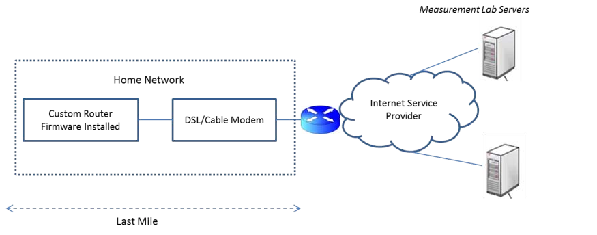
\includegraphics[width=0.5\textwidth]{gateway.pdf}
  % 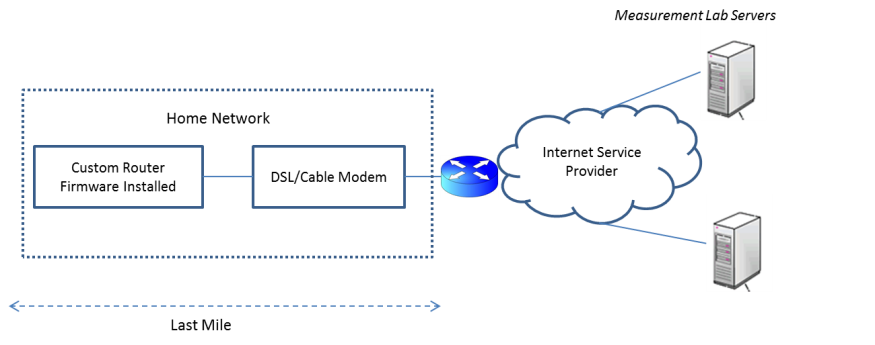
\includegraphics[height=0.2 \textheight,width=0.48 \textwidth]{gateway.png}
   \end {center}
 \caption{Gateway View for ISP measurement}
 \label {Fig:gateway}
\end{figure}


\begin {table}[h!]
\centering

 \begin{tabular}{|c|c|p{0.7in}|p{0.7in}|}
   \hline
   % after \\: \hline or \cline{col1-col2} \cline{col3-col4} ...
   \textbf{ISP} & \textbf{No of Users} & \textbf{Total Measurements} & \textbf{Latency measurements} \\
   \hline
   PTCL & \centering6 & 102396 &75665 \\
   \hline
   \centering WiTribe& \centering 3 & 260190 & 188572 \\
   \hline
   \centering Wateen & \centering 3 & 54661 & 39918 \\
   \hline
   \centering Qubee & \centering 1 & 180939 & 126083 \\
   \hline
   \centering Nayatel &\centering 2 & 127443  & 173002 \\
   \hline
 \end{tabular}
 \caption {Custom router deployment against ISP and users}
  \label {Table:2}
 \end {table}


\subsection {Collection period}
We collected data sets from September, 2013 till Mid-January 2014 in Pakistan (see Table \ref{Table:1}). We collected data from both fixed land line and wireless broadband connections for a given period of time using custom routers in collaboration with project BISmark ~\cite{29}. Measurements for different ISPs differ from each other as user behavior to turn on or off the router vary. When router is "ON", it reports to the server.\\
\textbf{Custom Router}\\
\indent In order to achieve our goals, we deployed 15 routers across different regions in Pakistan. These routers provide a sample of traffic for three major provinces of Pakistan including Punjab, KPK, and Federal Capital Territory. These routers are deployed at residential sites. Each site is equipped with a custom router. These routers are deployed in a fashion that they cover all major landline and fixed wireless broadband ISPs. They cover almost all variants of technology providing broadband in Pakistan, from Digital Subscriber Line to WiMax (IEEE802.16d). These routers take throughput and latency measurements continuously over time and report back to a measurement server, established at Islamabad, Pakistan. Along with deploying routers, we also distribute questionnaire among users, asking about their broadband service plans, their current experience and remarks about Internet speeds.  We manage these routers through online custom upgrades via a management server located at Georgia Institute of Technology, USA. Continuous measurements are performed by routers (see Table \ref{Table:2}). Latency measurements were performed against different measurement lab servers present across the world.
Primarily developed framework is categorized as:
\begin{itemize}
  \item We deployed 15 programmable OpenWrt routers (Thanks to Project BISmark for providing these routers) on home gateway router among different users having different ISP’s and service plans. These routers are mainly deployed in Islamabad, Rawalpindi, Wah cant and northern Pakistan. Islamabad and Rawalpindi were considered as privileged sites.
  \item A measurement server is established at NUST, SEECS, against which the measurements were performed. Measurement server reports to management server at Georgia Tech USA.
  \item The measurements which we took were: Upload throughput, download throughput, Latency, Jitter etc
  \item In order to collect the dumps of said measurements, shell script is burned on programmable routers to measure which execute automatically for different spans of time.
  \item Latency measurements (ms) are taken using ping to a set of servers across the globe; once every 10 minutes, similarly last mile latency as well. 
  \item Upstream and downstream throughputs (kbits/s) are taken by using NETPERF. About once every 2 hours (also depends on server load), and alternates between using 1 and 3 parallel TCP threads.
  \item Creating MYSQL database asynchronously, after parsing the attributes.
  \item Generating Results for broadband performance measurements.
\end{itemize}


\subsection{Challenges}
Challenges are always an integral part of work, specifically in third world countries like Pakistan. The most pressing challenge is having most of the customer plans with data caps on their broadband connections. In most of the cases, customers tend to blame custom routers for exceeding data cap limits which may not exactly be the case. This limits extent of data sent from user devices to server. Thus, it is important to carefully select data for sending to the server. Most frequent measurements may give in depth insights but result in exhausting data cap for a user, thus appropriate tradeoff needs to be maintained.\\
\indent	 Second, we had to ensure routers are "ON" for most of the time. Users tend to unplug the devices when not in use. We had to engage users in the study in order to keep devices "ON" with frequent follow ups through email, phone and personal contacts. We had to ensure that our devices do not interrupt users' Internet access and take measurements for a short span of time (typically less than 15 sec).\\
\indent Another significant challenge was user's privacy concerns. Most of the users were concerned about their privacy. In order to engage users in the study, data collected from user devices is also made available to them so they can download their data gathered by routers. This allayed some of the user concerns giving them surety that no browsing data is recorded.

\section {RESULTS}
In this section, we share the results of our study. First, we present whether broadband ISPs, fixed land line and wireless, fulfill promise of service advertised to customers. Subsequently, we investigate steadfastness in performance and other factors that affect performance, such as latency to different international servers and services.
We observed fixed (landline and wireless) broadband for five major broadband service providers in our dataset. To complement, we take feedback from users regarding their broadband speeds through email questionnaires.
\subsection { Downlink Throughput of Broadband ISP's in Pakistan:}
\indent By use of our custom routers data, first we study whether throughput of different router tools matches advertised rate, claimed by ISPs to clients. For this purpose, we use concept of normalized throughput: throughput attained by customer divided by throughput advertised by ISP for a given service plan. Figure \ref{Fig:normalized} shows normalized throughput for each of the broadband service providers present in our data sets. (The caption below figure shows how to interpret boxplot). As results indicate, most of the ISPs fall below their advertised rates. In some rare occurrences, throughput measurements went over advertised rates as shown by whiskers in plot.
\begin{figure}[t!]
\begin {center}
   %Requires \usepackage{graphicx}
   %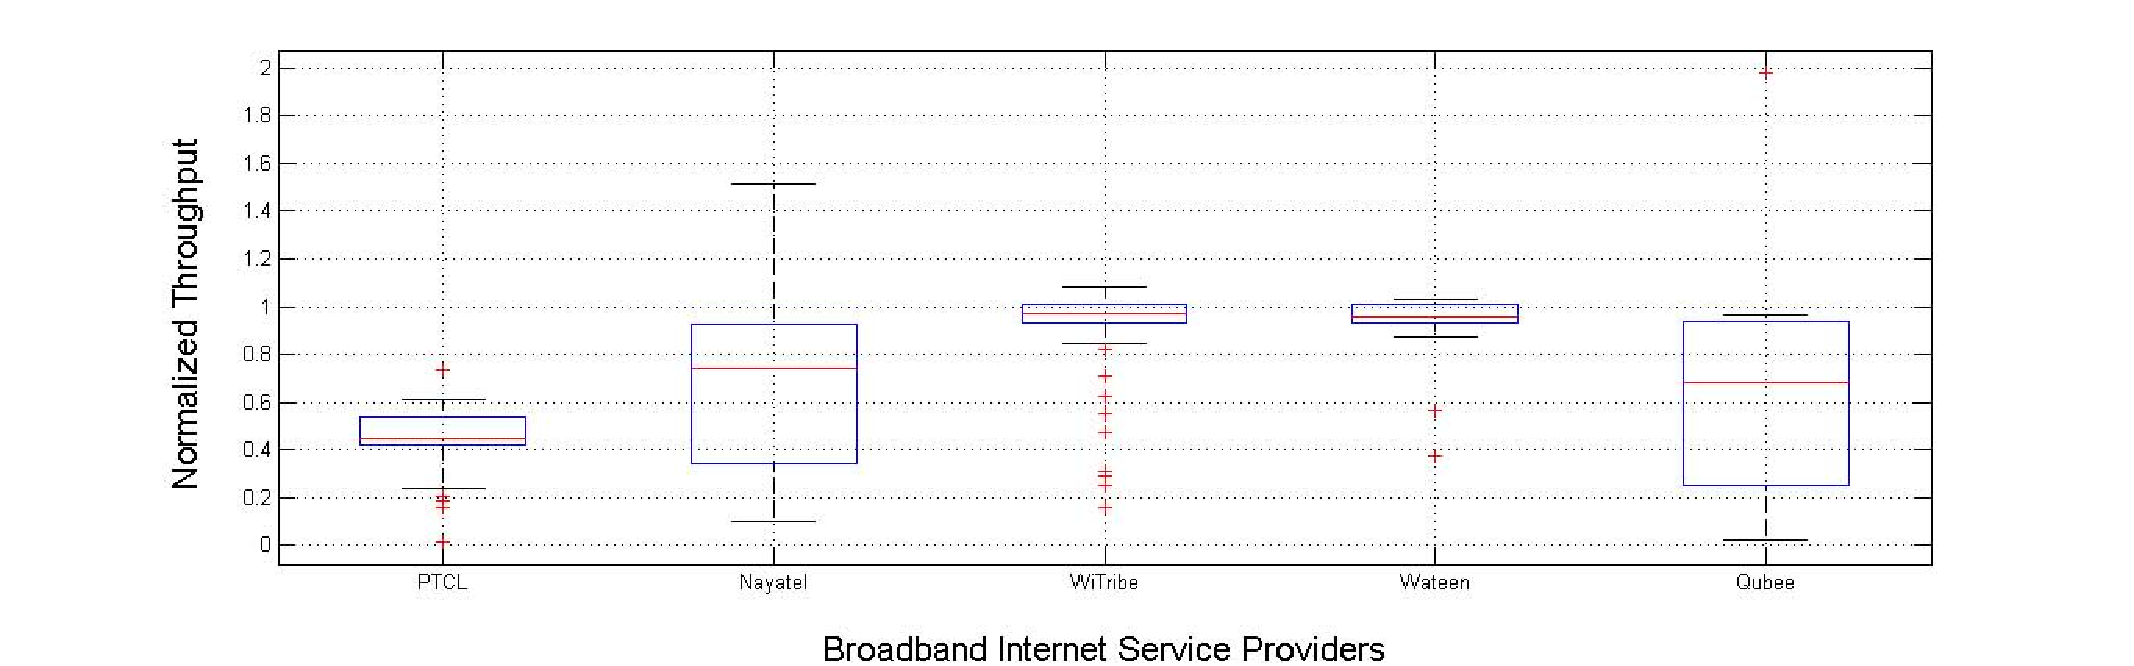
\includegraphics[height=0.2 \textheight, width=0.5\textwidth]{normalized.pdf}
   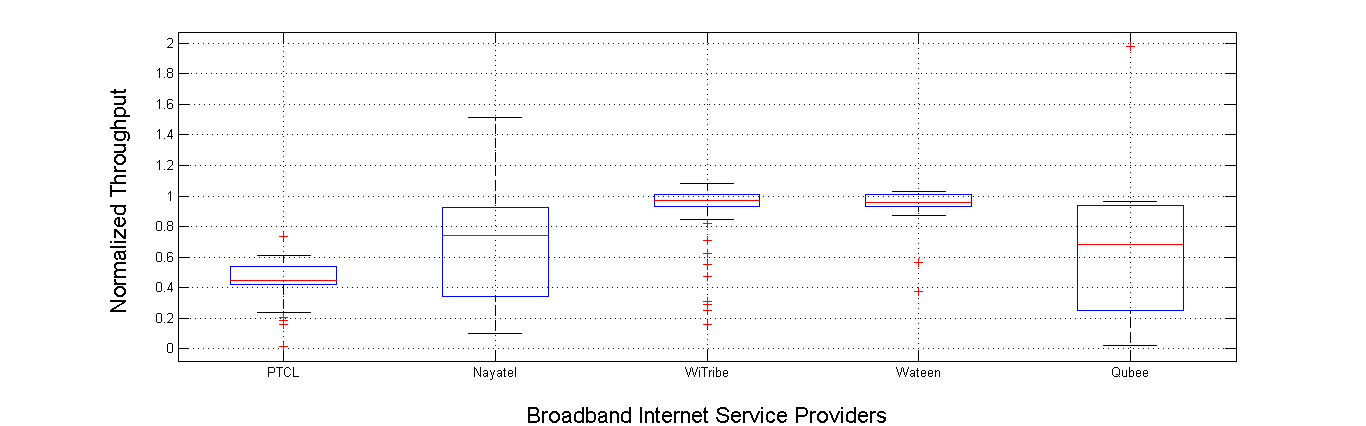
\includegraphics[height=0.2 \textheight,width=0.5 \textwidth]{normalized.png}
   \end {center}
 \caption{Throughput of each ISP normalized by rate advertised according to service plan (Value of 1 means advertised rate meets the attained throughput). The box shows interquartile range whereas red line shows median value and whiskers show 10th and 90th  percentile values. \emph{\textbf{Results shows most of the ISPs fall well below the advertised rates}}.}
\label{Fig:normalized}
\end{figure}


\begin{figure}[t!]
\begin {center}
   %Requires \usepackage{graphicx}
   %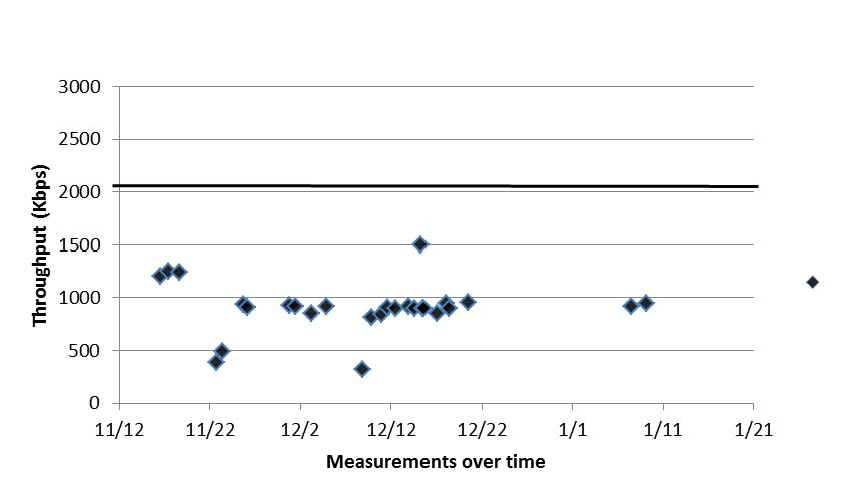
\includegraphics[width=0.5\textwidth]{3.pdf}
   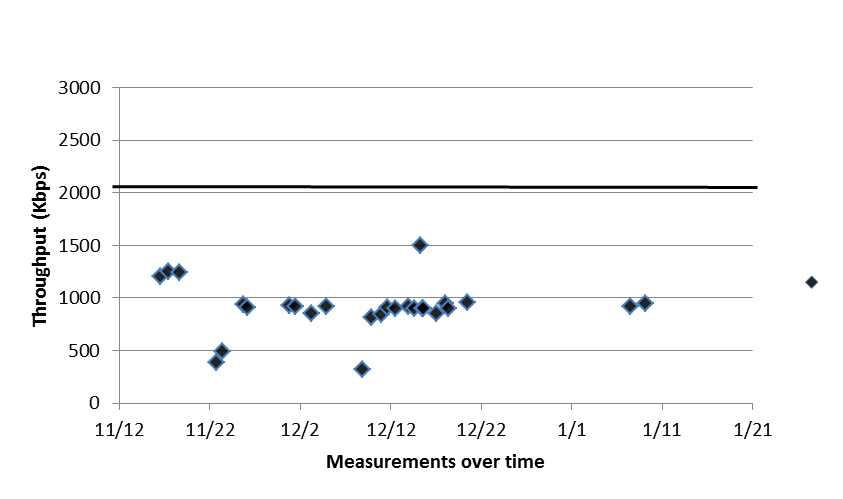
\includegraphics[height=0.2 \textheight,width=0.5 \textwidth]{3.png}
   \end {center}
 \caption{Timeline of throughput measurements from a PTCL user, in North Pakistan over a course of time. The advertised downstream throughput for this user is 2Mbps (2048 Kbps). Unfortunately the users only get 1Mbps during the entire time.}
 \label{Fig:3}
\end{figure}

\indent For further analysis, we investigate different grievous cases where advertised rate does not meet attainable rates. Figure \ref{Fig:3} shows time line of throughput measurements for almost three months for one of the case. In this case, ISP advertised service plan was of 2 Mbps though results so attained are well below advertised rate (less than half).  This case falls under one of the extreme cases we analyzed.
 Similarly, from our data collection, we also study distribution of latencies from different service providers to measurement server. Figure \ref{Fig:4} gives box and whisker plot of latencies for different ISPs, y-axis is log scale. These values envisage farfetched variable latencies and in some cases very high latency values, as shown by whiskers in Figure \ref{Fig:4}.

\begin{figure}[t!]
\begin {center}
   %Requires \usepackage{graphicx}
   %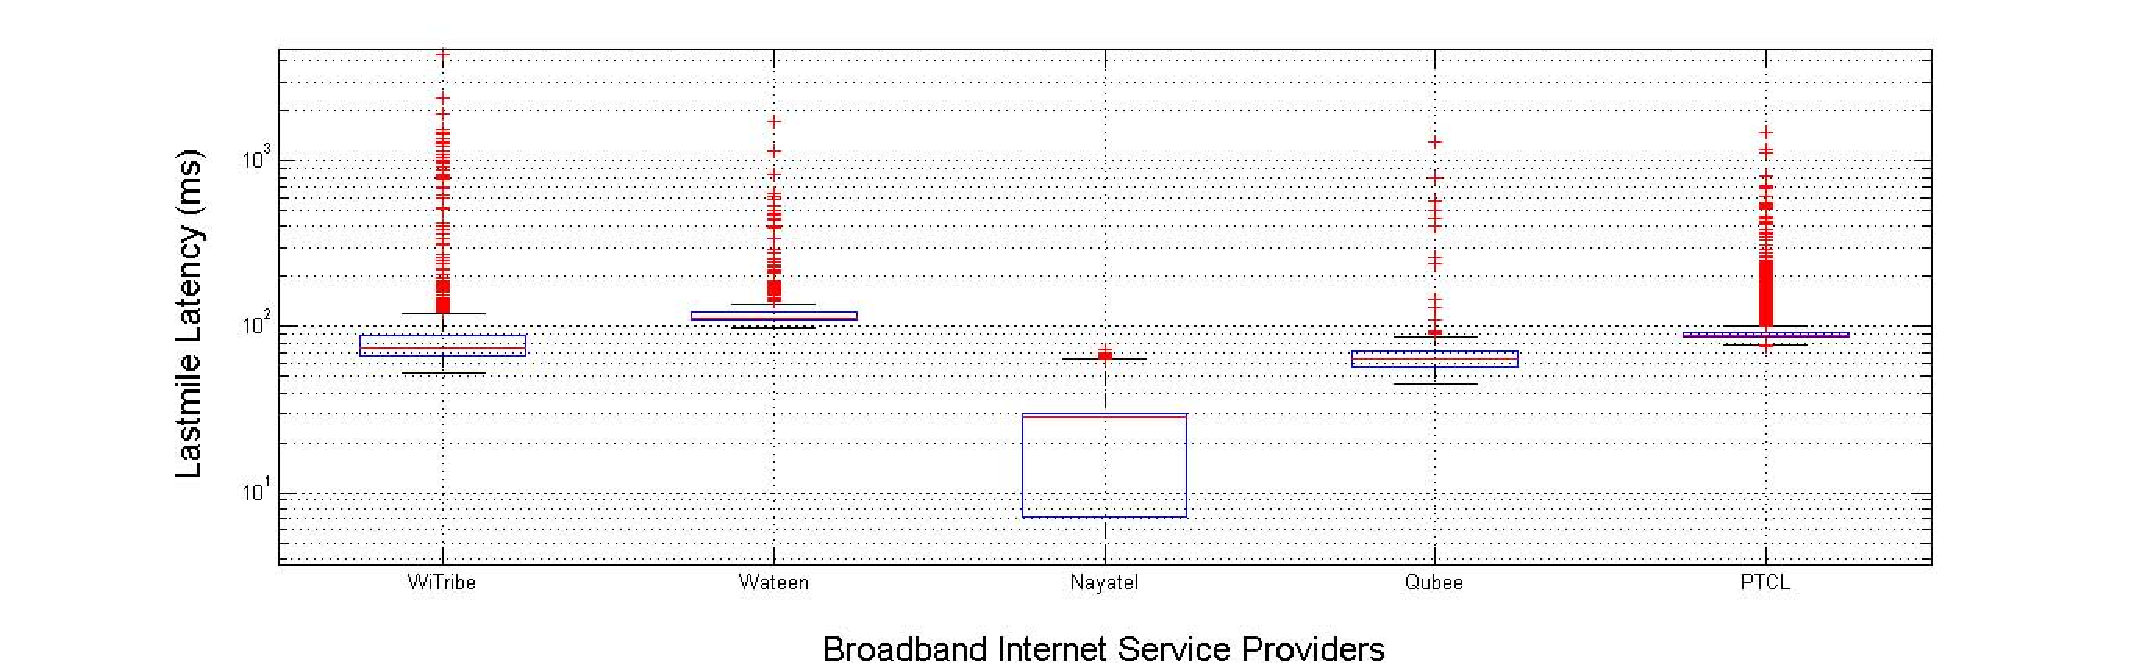
\includegraphics[height=0.2 \textheight, width=0.5\textwidth]{4.pdf}
   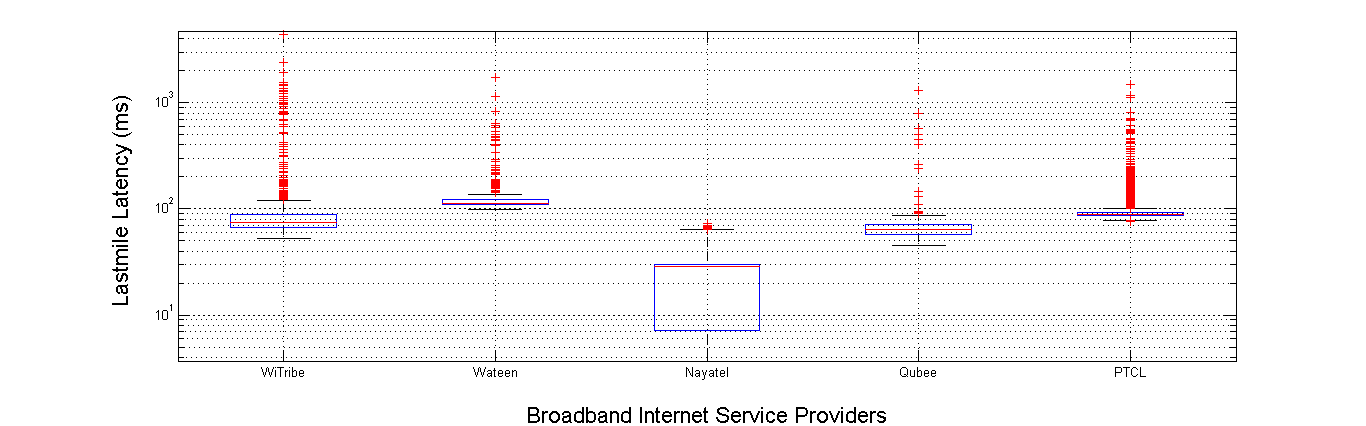
\includegraphics[height=0.2 \textheight,width=0.5 \textwidth]{4.png}
   \end {center}
 \caption{The latencies for each ISP to server at Islamabad, Pakistan. The boxes shows the Interquartile range whereas redline show the median and the whiskers show the 10th and 90th percentiles. Y-axis is logarithmic scale. The red lines over the whiskers are outliers.}
 \label{Fig:4}
\end{figure}

\subsection {Fixed Wireless Broadband Performance:}
\indent From our dataset, we calculate downstream throughput for different fixed wireless broadband service providers against local server at Islamabad, Pakistan and also against an international server at London, United Kingdom. Figure \ref{Fig:5} shows results of downstream throughput against local server whereas Figure \ref{Fig:6} shows result of downstream throughput against the international server. The results clearly depict that interquartile ranges for different wireless broadband ISPs are not that large. There is very less variation in download throughput for both cases. Qubee has larger interquartile range than Wateen and WiTribe showing greater variations. Similarly, download throughput against local server is greater for all ISPs with fewer variations whereas against international server, download throughput is less in comparison with local server. Also, greater variations in download throughput are observed for international server (London).

\begin{figure}[t!]
\begin {center}
   %Requires \usepackage{graphicx}
   %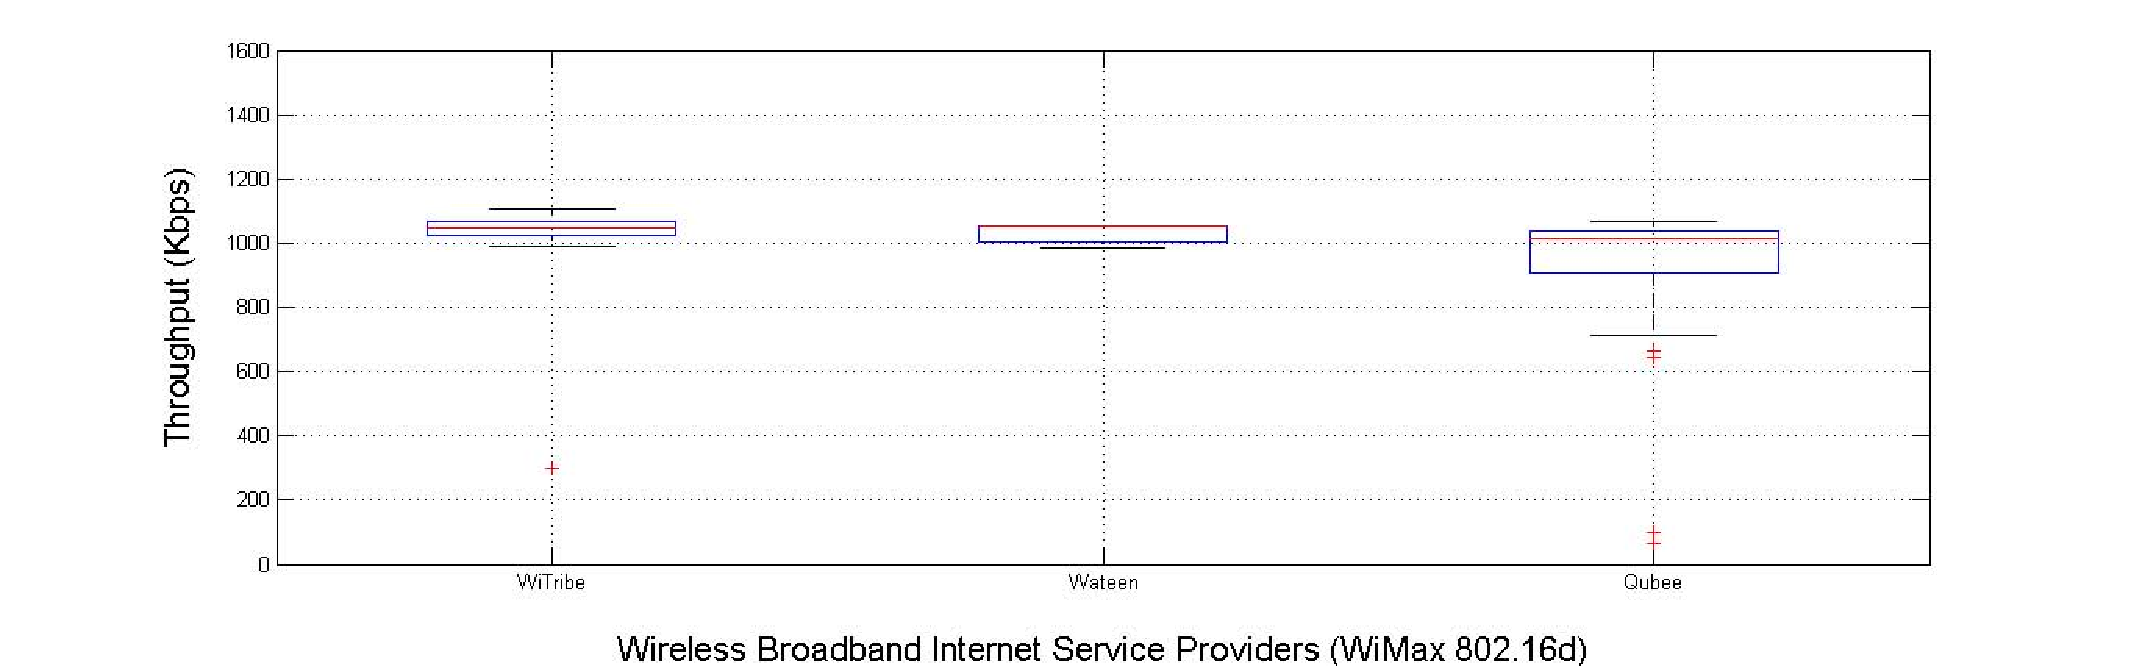
\includegraphics[height=0.2 \textheight, width=0.5\textwidth]{5.pdf}
   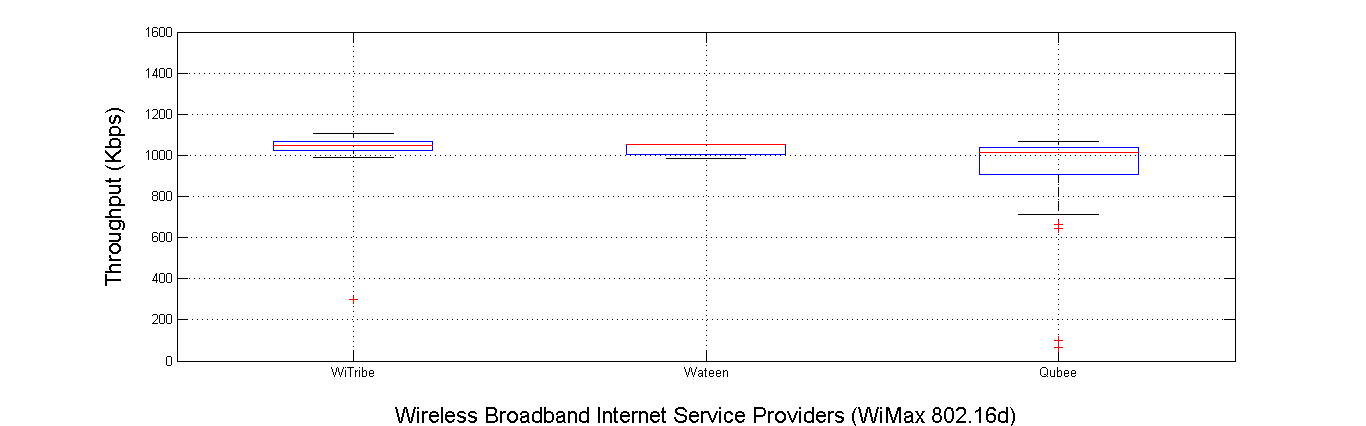
\includegraphics[height=0.2 \textheight,width=0.5 \textwidth]{5.png}
   \end {center}
 \caption{Download throughput for different Wireless broadband ISPs against the local server at Islamabad, Pakistan.Nearly all the ISPs experience the same throughput.} \label{Fig:5}
\end{figure}
\begin{figure}[t!]
\begin {center}
   %Requires \usepackage{graphicx}
   %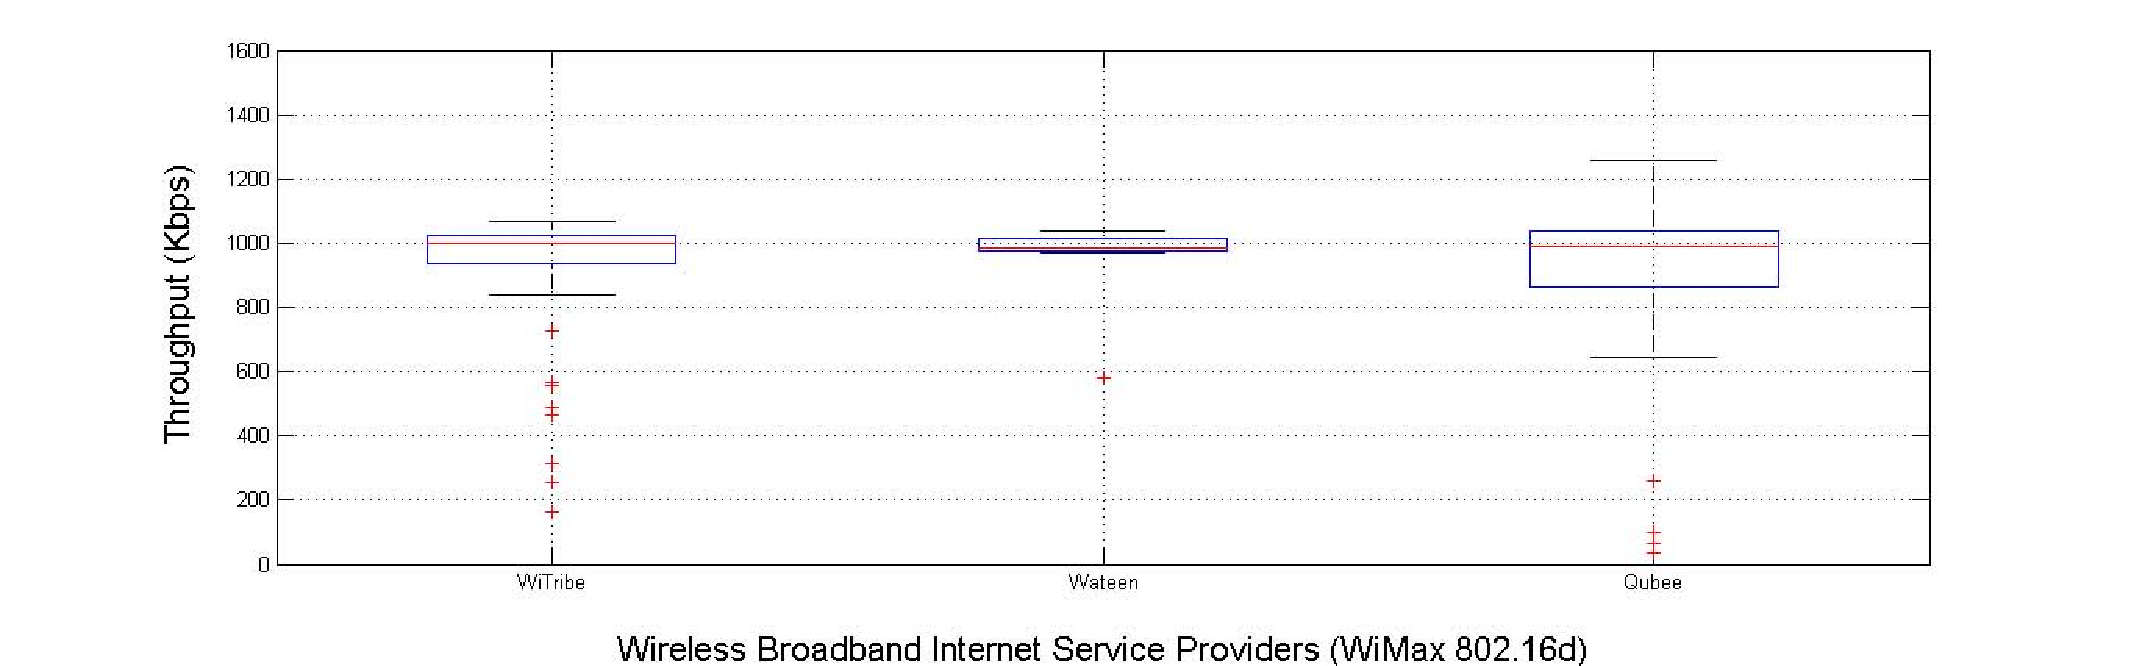
\includegraphics[height=0.2 \textheight, width=0.5\textwidth]{6.pdf}
   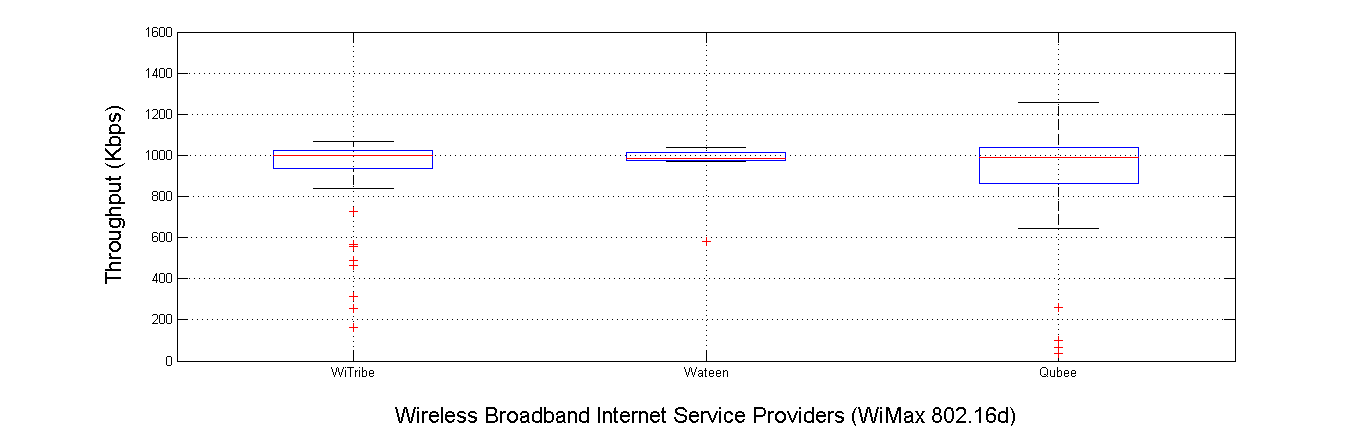
\includegraphics[height=0.2 \textheight,width=0.5 \textwidth]{6.png}
   \end {center}
 \caption{Download throughput for different Wireless broadband ISPs against the International server in London. Nearly all the ISPs experience same throughput but little less than that of local server.} \label{Fig:6}
\end{figure}

%\textbf{Upload speeds}\\
%\indent Upload throughput of all ISPs available in our data set is plotted in Figure \ref{Fig:7}. The upload speed for WiTribe, Wateen, Qubee is plotted %against their service plan of 1 Mbps whereas PTCL is plotted against service plan of 2 Mbps and Nayatel against 3 Mbps. These are service plans for download %throughput and upload is not usually defined in the plan. Customers usually care less about upload speeds unless highly constrained. Nayatel provides maximum %upload throughput with larger interquartile range, showing a lot of variations, whereas remaining ISPs with small interquartile ranges show less variations and %nearly constant upload throughput values.

%\begin{figure}[t!]
%\begin {center}
   %Requires \usepackage{graphicx}
   %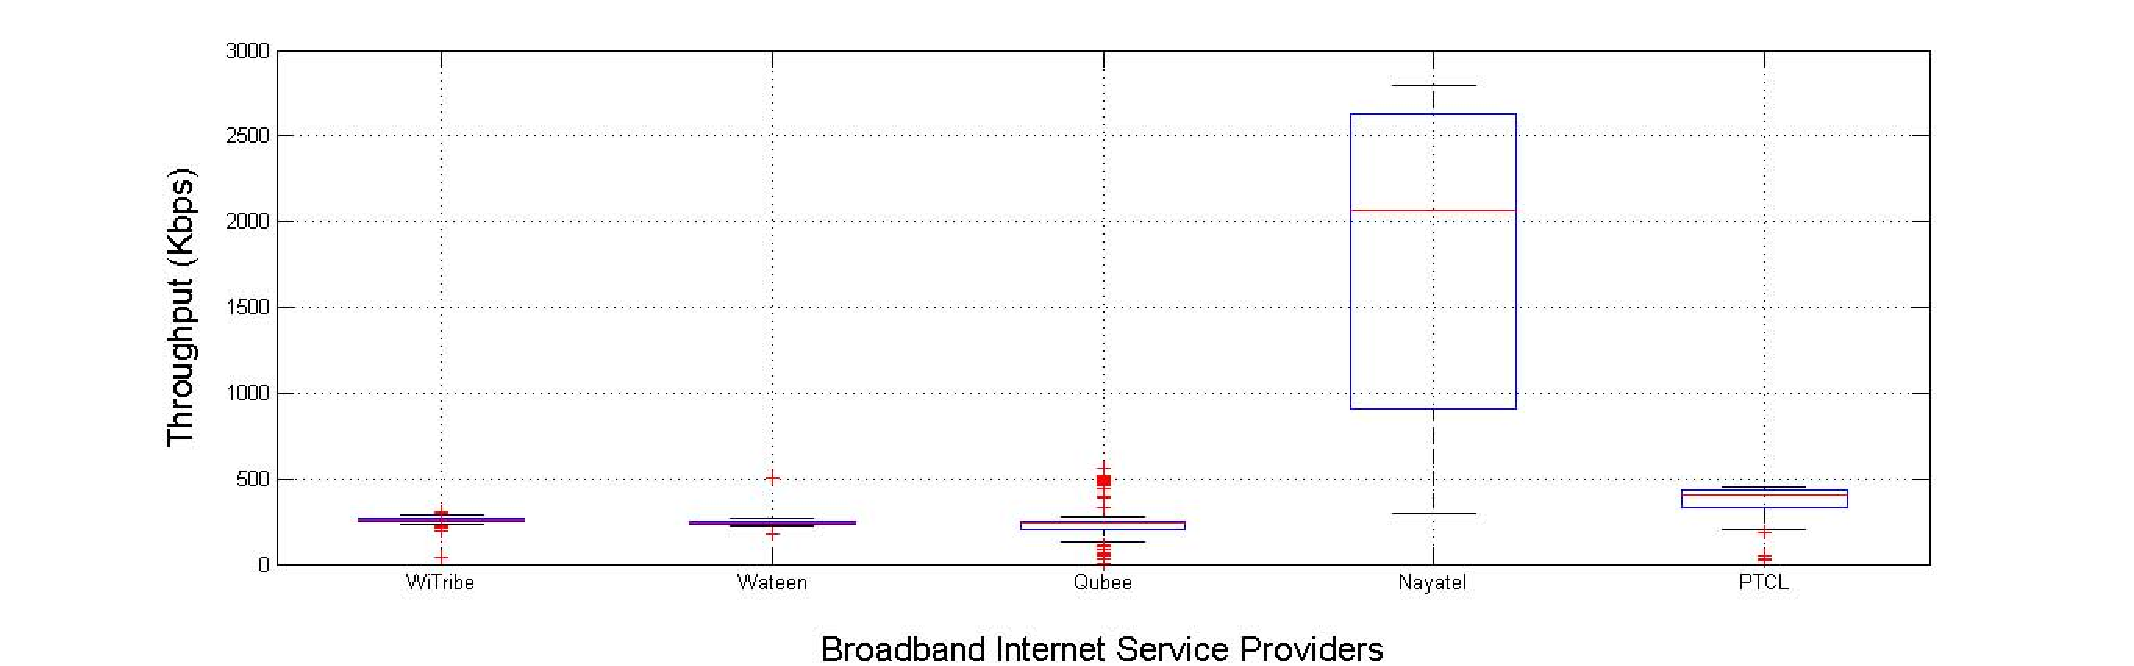
\includegraphics[height=0.2 \textheight, width=0.5\textwidth]{7.pdf}
 % 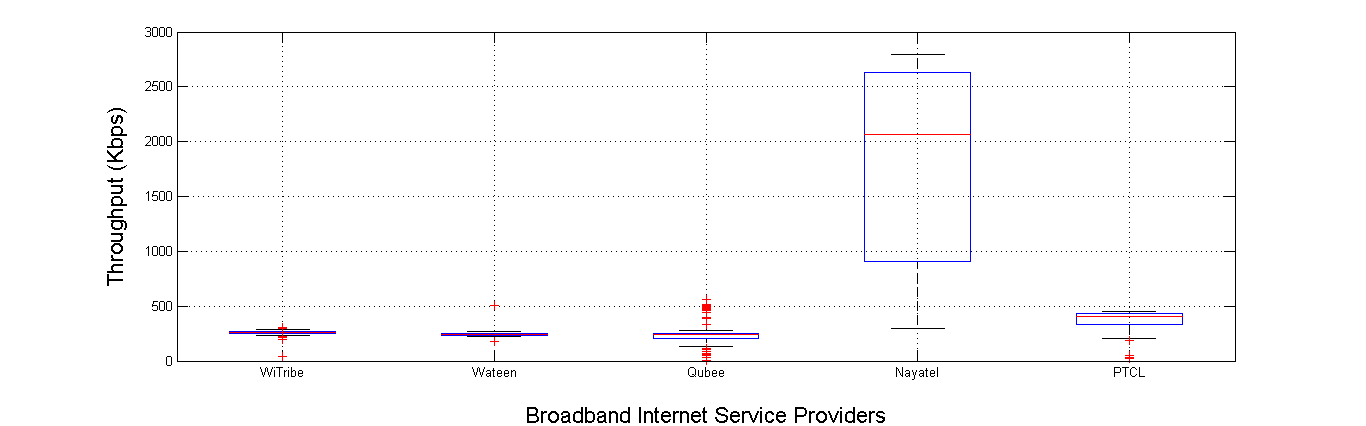
\includegraphics[height=0.2 \textheight,width=0.5 \textwidth]{7.png}
 %  \end {center}
% \caption{Upload throughputs of different broadband ISPs .} \label{Fig:7}
%\end{figure}
\subsection {Reliability Test: Land line vs Fixed Wireless}
The comparison between fixed (landline and wireless) providers is to be made by considering following scenario. Both land line and wireless broadband ISPs are tested for throughput measurements from same location to measurement server at Islamabad, Pakistan.
\begin{figure}[t!]
\begin {center}
   %Requires \usepackage{graphicx}
   %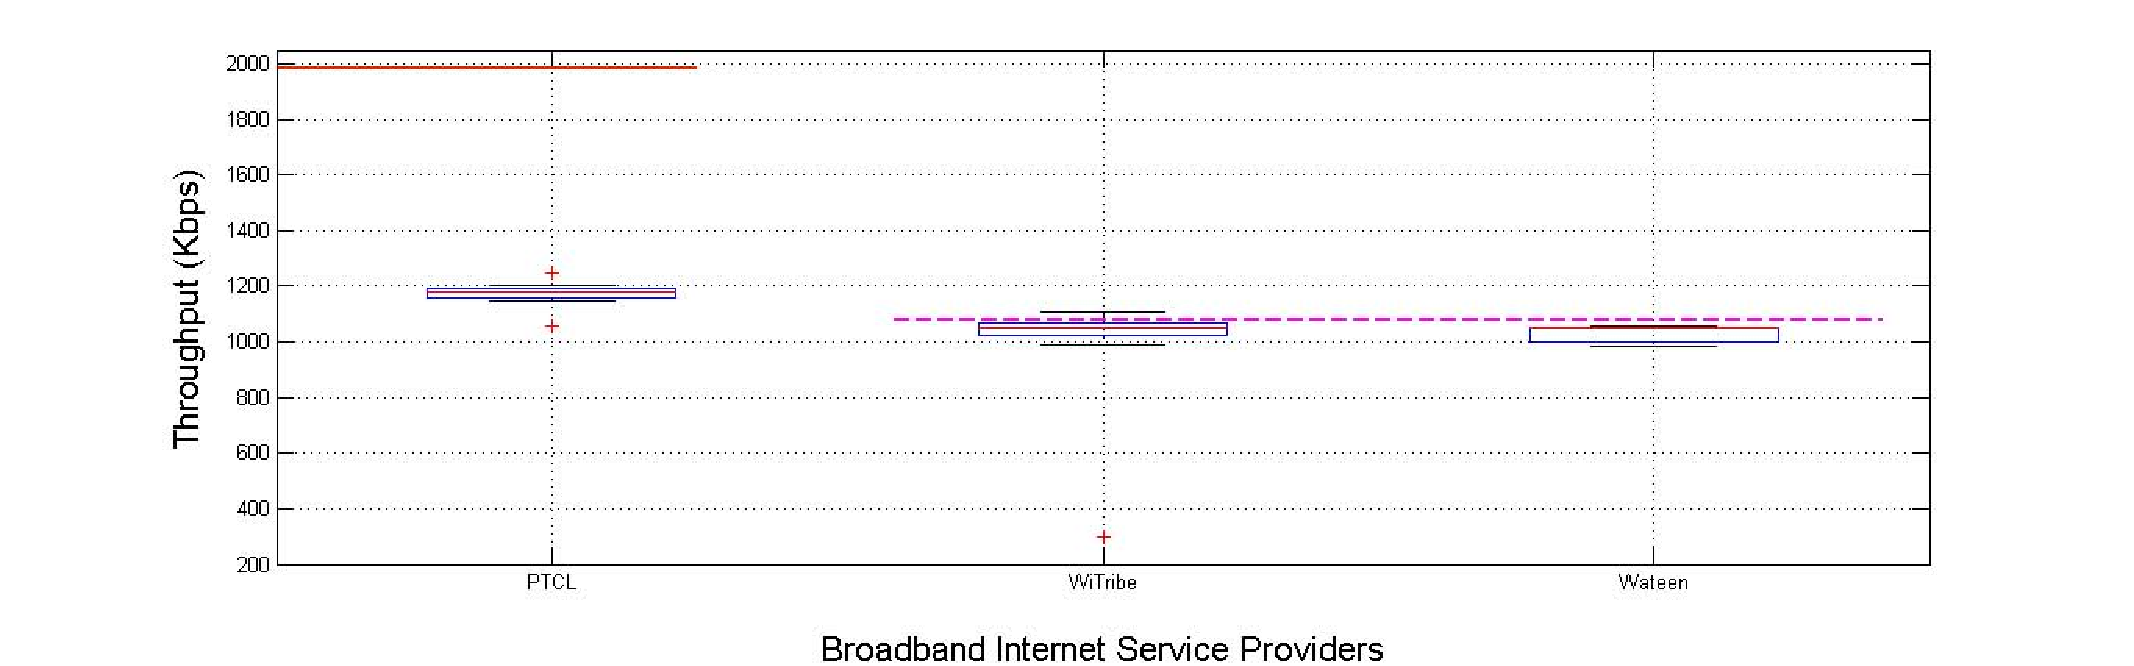
\includegraphics[height=0.2 \textheight, width=0.5\textwidth]{8.pdf}
  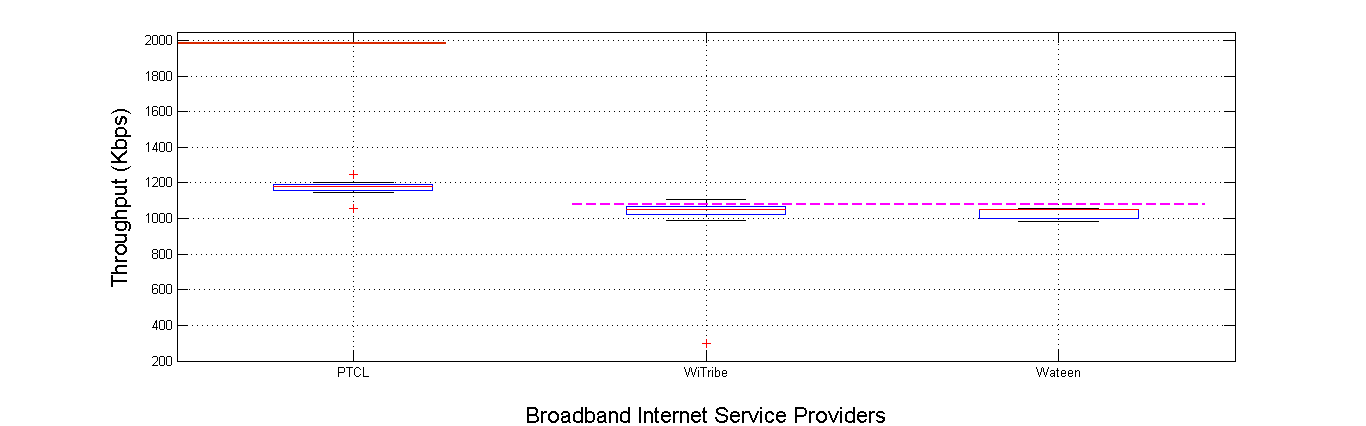
\includegraphics[height=0.2 \textheight,width=0.5 \textwidth]{8.png}
   \end {center}
 \caption{Downstream throughput measurements of one fixed land line (PTCL) and two wireless (WiTribe and Wateen) fixed broadband from same geographic location to measurement server at Islamabad, Pakistan. The red line above PTCL shows service plan against which it is plotted, similarly dotted line above WiTribe and Wateen. The fixed landline throughput is considerably lower than wireless broadband (Fixed)} \label{Fig:8}
\end{figure}
Figure \ref{Fig:8} gives throughput measurements from same location to measurement server whereas Figure \ref{Fig:9} gives latency measurements from same location to measurement server. Figure \ref{Fig:8} clearly depicts that for a region where both fixed land line and wireless (Fixed) broadband is available, wireless outperforms fixed land line.\\
\indent Figure \ref{Fig:9} shows distribution of latency measurements. Key take away here is that latency for landline is also higher than that of wireless broadband. Y-axis is log scale, hence even small change is prominent.

\begin{figure}[t!]
\begin {center}
   %Requires \usepackage{graphicx}
   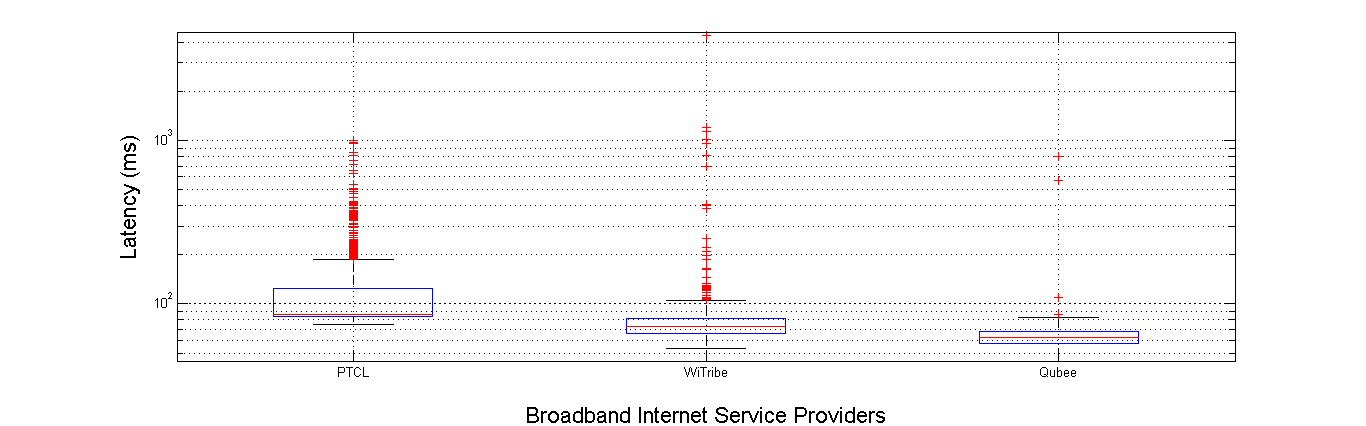
\includegraphics[height=0.2 \textheight,width=0.5 \textwidth]{9.png}
   %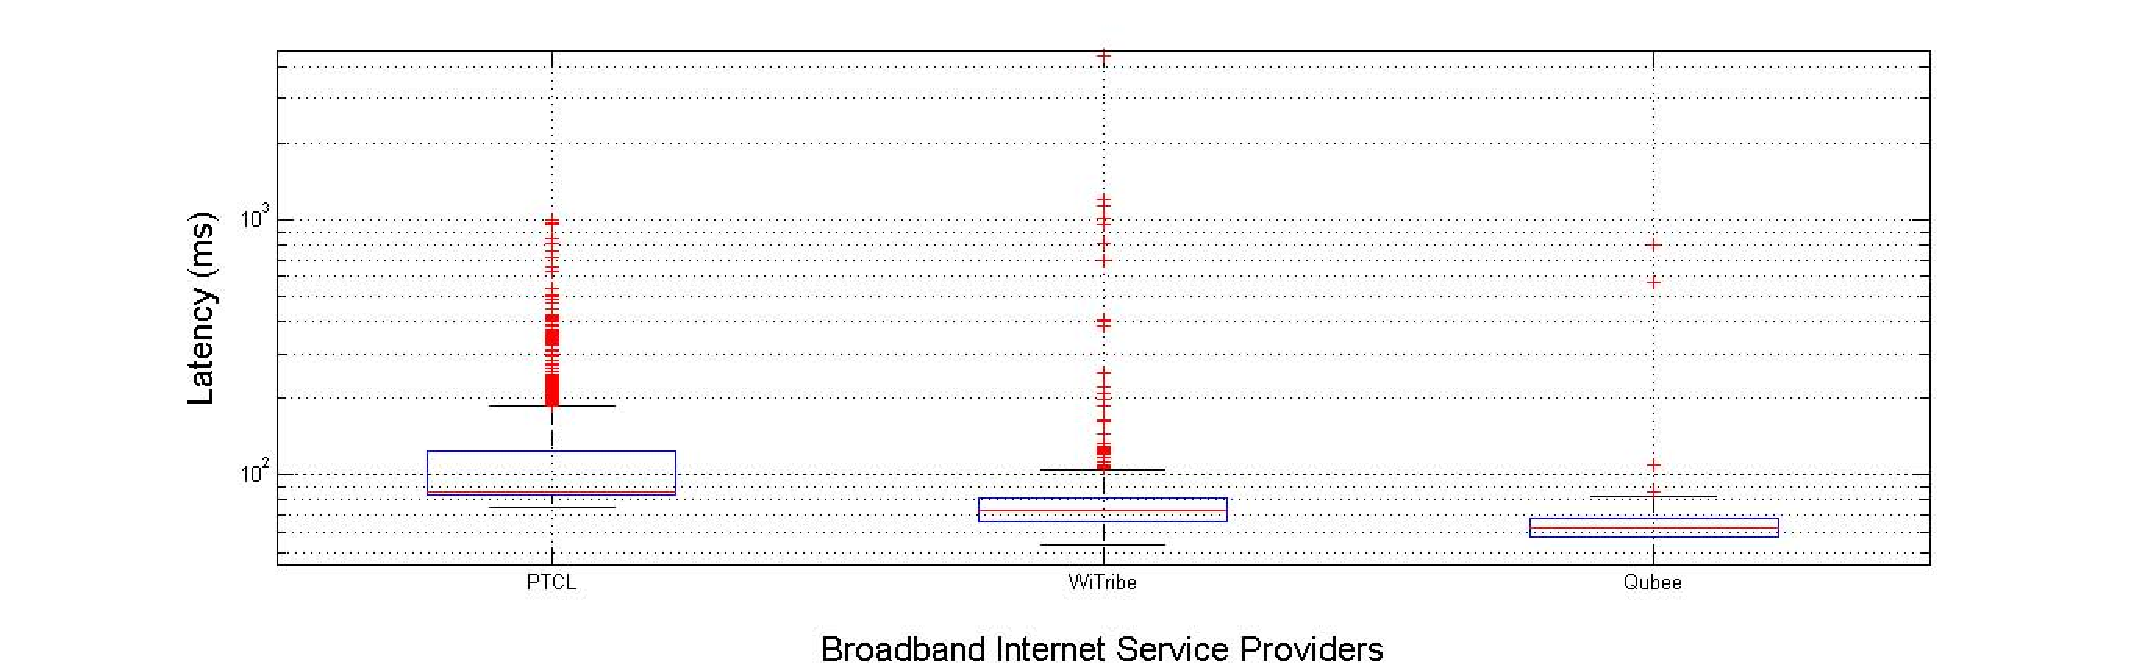
\includegraphics[height=0.2 \textheight, width=0.5\textwidth]{9.pdf}
   \end {center}
 \caption{Latency measurements for one fixed land line (PTCL) and two wireless broadband (WiTribe \& Wateen) from same geographic location to measurement server at Islamabad. Y-axis is log scale. Fixed land line experiences high latency values than wireless broadband.}\label{Fig:9}
\end{figure}

PTCL is the dominant broadband service provider in Pakistan, we picked up customers from different regions and plotted throughput against their service plan in order to see whether PTCL performance degrades overall (see Figure \ref{Fig:10}). Similarly in Figure 2, we used the concept of normalized throughput. A result clearly depicts that most of the PTCL customers are not attaining rates which PTCL promises.
\begin{figure}[t!]
\begin {center}
   %Requires \usepackage{graphicx}
   %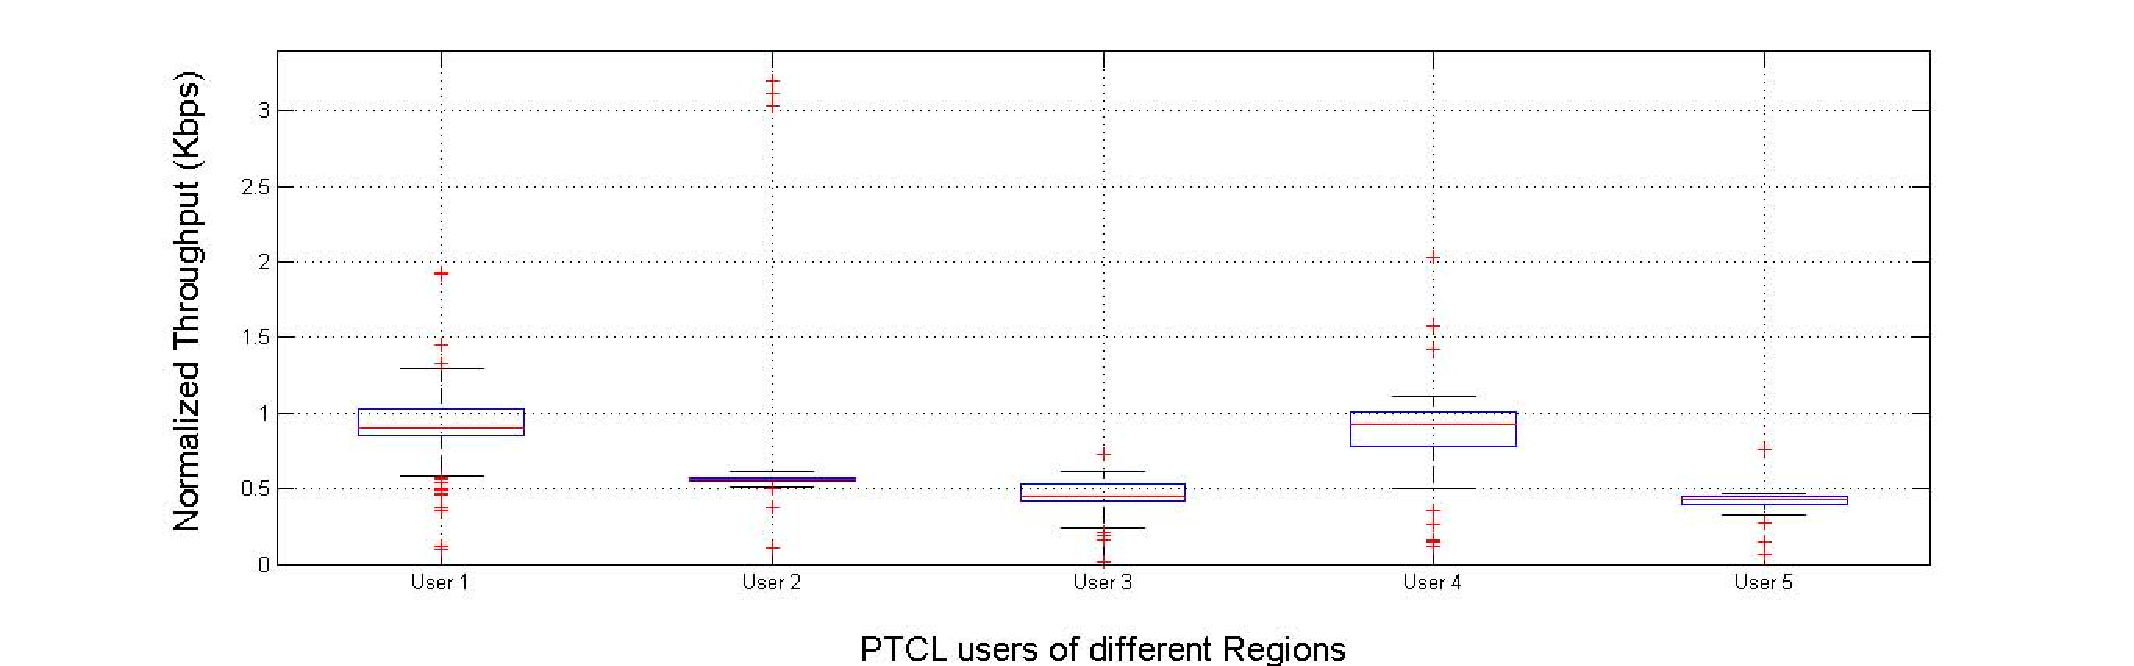
\includegraphics[height=0.2 \textheight, width=0.5\textwidth]{15.pdf}
      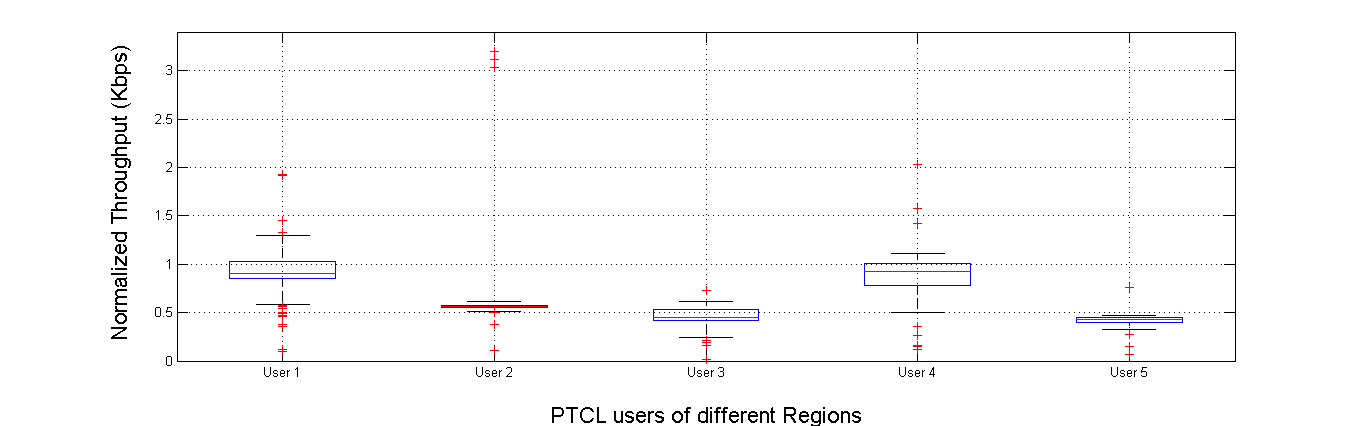
\includegraphics[height=0.2 \textheight,width=0.5 \textwidth]{15.png}
   \end {center}
 \caption{Normalized throughput of PTCL users from different regions. Throughput of the users is normalized by the rate advertised to them. 1 means attained rate is equal to advertised rate} \label{Fig:10}
\end{figure}

\indent In order to compare fixed land line and wireless broadband, we also plot downstream throughput in terms of cumulative distribution function. Figure \ref{Fig:11} gives cumulative distribution function of various technologies used in our custom router data set. Results clearly depict that WiMax IEEE802.16 d provides better throughput measurements than that of Asymmetric Digital Subscriber line (ADSL) in regions where both are available. Nayatel (FTTH) also performs well but its coverage is only in capital city Islamabad, Pakistan.  This performance aspect can be attributed as one of the main reasons for rapid growth of WiMax in Pakistan ~\cite{28} where both fixed line and wireless are available.

\begin{figure}[t!]
\begin {center}
   %Requires \usepackage{graphicx}
   %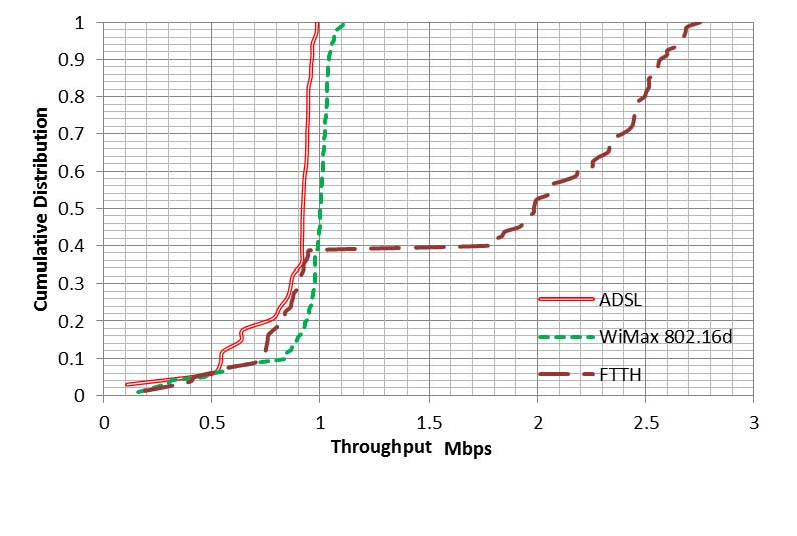
\includegraphics[ width=0.5\textwidth]{10.pdf}
   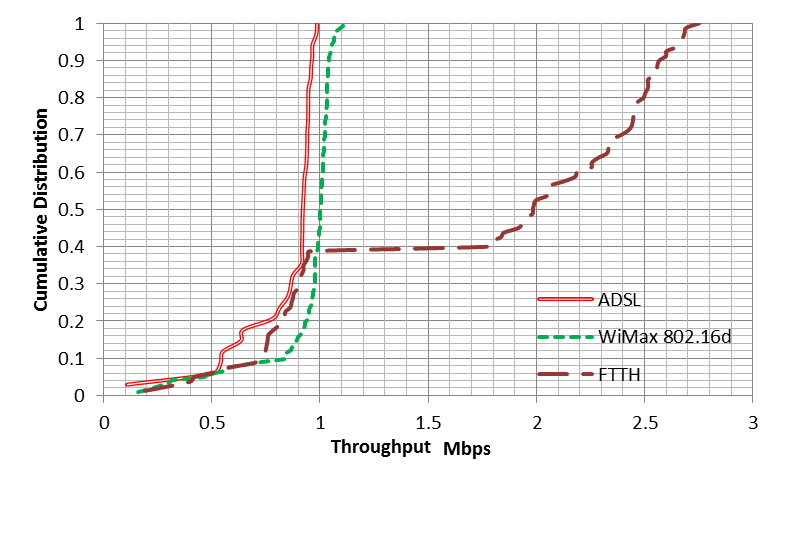
\includegraphics[height=0.2 \textheight,width=0.5 \textwidth]{10.png}
   \end {center}
 \caption{Cumulative distribution of download throughput of different fixed landline and wireless technologies in our dataset. FTTH is plotted against the service plan of 3 Mbps whereas ADSL against 2 Mbps and WiMax against 1 Mbps. WiMax and FTTH give higher throughput than ADSL.} \label{Fig:11}
\end{figure}


%\begin{figure}[h!]
%\begin {center}
   %Requires \usepackage{graphicx}
 % 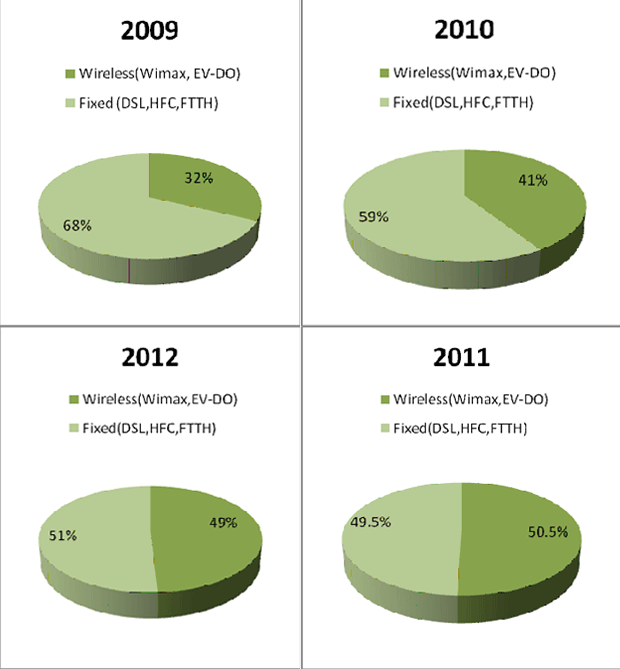
\includegraphics[height=0.2 \textheight,width=0.5 \textwidth]{11.png}
 %\end {center}
%\caption[Market share for service providers in Pakistan]{Market share for service providers in Pakistan~~\cite{28}}
%\label{Fig:12}
%\end{figure}

\indent To summarize results of router based measurements, most of the ISPs do not appear to fulfill QoS demands they claim. WiMax outperforms landline (ADSL) where both are available.

\subsection {Investigating other factors that affect performance:}
Now we look how factors such as distance of international servers, time of day when user uses broadband connection and latency to popular services affect   performance of broadband connection. Surprisingly, we found that users attain degraded performance to popular websites and services because of high values of latency as various servers have high latency path to Pakistan. This high value of latency may not mean that geographically, these servers are far away. Connectivity between different ISPs is not as dense in Pakistan as in other areas of the world. These subjects are discussed in detail further below.

\subsubsection {Latency to various measurement lab servers)}
Figure \ref{Fig:13} gives the average latencies to measurement lab servers around the world from custom router users. The bars in Figure \ref{Fig:13} give average latencies and numbers with name of city showing distance from Islamabad. The bars are sorted in an increasing distance from Islamabad. Fascinatingly, values of latency do not depend upon geographic distance. For example latency to New Delhi is around 300 to 400 millisecond which is only 686 Kilometers away but latency to London is around 200 to 300 millisecond which is 6040 Kilometers away. The results depict that European destinations are 7 to 8 times farther away from Pakistan relative to New Delhi but their latency values are less as compared to New Delhi. In order to investigate paths, we use trace-route network measuring tool which traces paths of routed traffic. In case of New Delhi, India, Pakistan does not have any direct route with ISPs in India, all traffic routed to India is via Singapore exchange point. Thus, direct exchange points are required between different ISPs in Pakistan and India to reduce latency measurements. Similarly, in case of Nairobi, Cape Town and Rio de Janeiro, there are no direct routes. Traffic to Nairobi, Cape Town and Rio de Janeiro is routed via European Exchange Points. Thus a direct routes along with ISPs collaboration and peering is required to reduce latency values.
 \begin{figure}[t!]
\begin {center}
   %Requires \usepackage{graphicx}
   %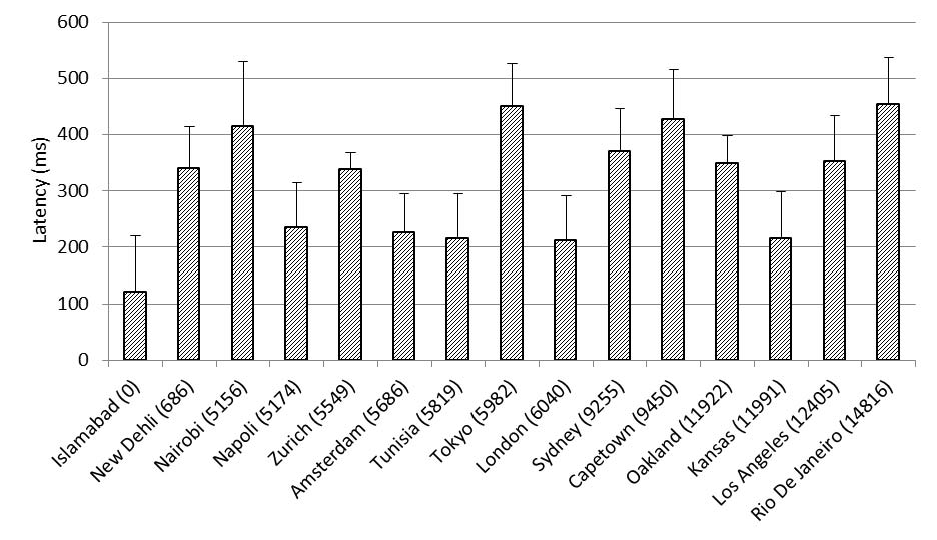
\includegraphics[ width=0.5\textwidth]{12.pdf}
   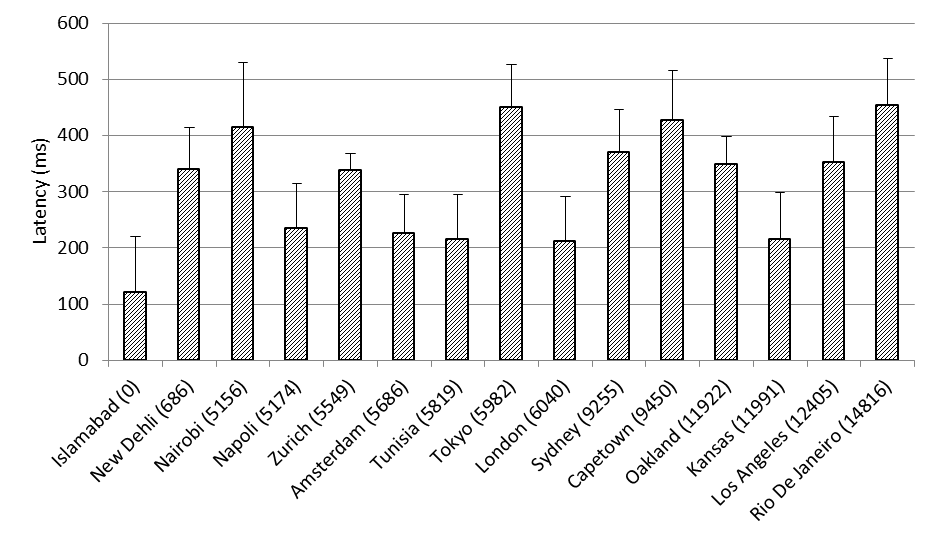
\includegraphics[height=0.2 \textheight,width=0.5 \textwidth]{12.png}
   \end {center}
 \caption{Mean latencies to the measurement lab servers around the world from Islamabad, Pakistan. Numbers along with the city name reflects the distance in kilometers from Islamabad. The bars are sorted as in increasing distance from Islamabad.}
 \label{Fig:13}
\end{figure}

\subsubsection{Alternative routes to global destinations:}
Traffic that is routed from Pakistan to global destinations effects not only performance but also reliability. Pakistan is connected to rest of the world via 4 submarine cables i-e SEA-ME-WE-4, SEA-ME-WE-3, IMEWE, and Transworld (TW1). When Trans-cable SEA-ME-WE-4 was cut on 27th march 2013 ~\cite{27}, it disrupted Internet services in Pakistan. The entire traffic was shifted to other Trans-cables. Figure \ref{Fig:14} shows increase in latencies observed during the period. This highlights the need for alternative routes on which traffic should be shifted in case of emergencies in order to make global services available in Pakistan with low latencies to international destinations. The measurement lab servers at different regions in Africa, North America were pinged to get the latency values.
\begin{figure}[t!]
\begin {center}
   %Requires \usepackage{graphicx}
   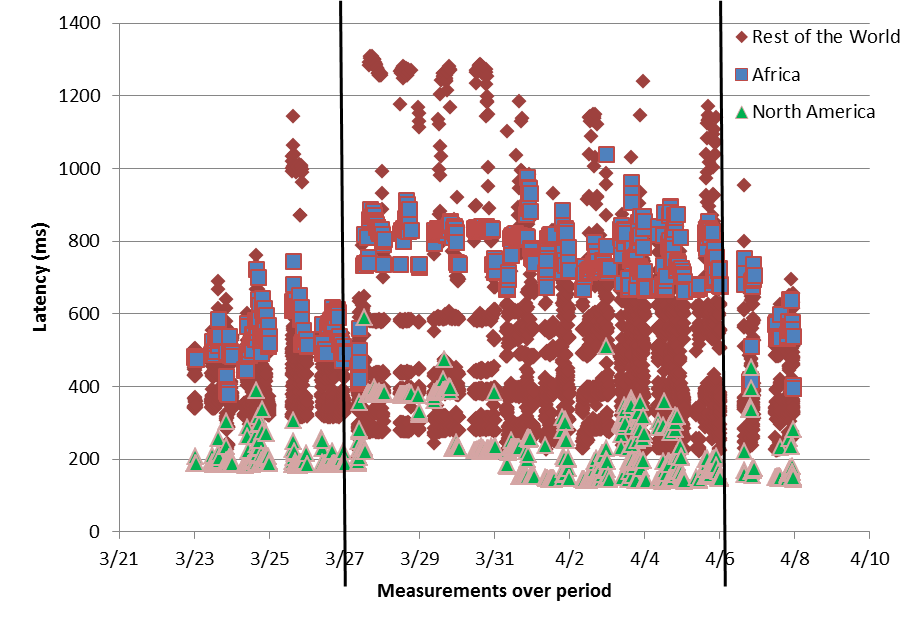
\includegraphics[height=0.2 \textheight,width=0.48 \textwidth]{13.png}
   \end {center}
 \caption{Increase in latencies values during the period when Trans-cable SEA-ME-WE-4 was cut.}\label{Fig:14}
\end{figure}
\subsubsection{Time of Day}
Previous studies have shown that local time of day affects network performance dramatically. This is because at peak hours, networks became more congested ~\cite{23} due to which performance is degraded. We analyzed whether same behavior is experienced in Pakistan or not.
We took measurements at different times of day against two different servers, one at Atlanta, US and other at Kansas, US (Google DNS). Figure \ref{Fig:15} shows latency against local time of the day.  Results depict increase in latencies and becoming more variable during peak hours.

\begin{figure}[t!]
\begin {center}
   %Requires \usepackage{graphicx}
   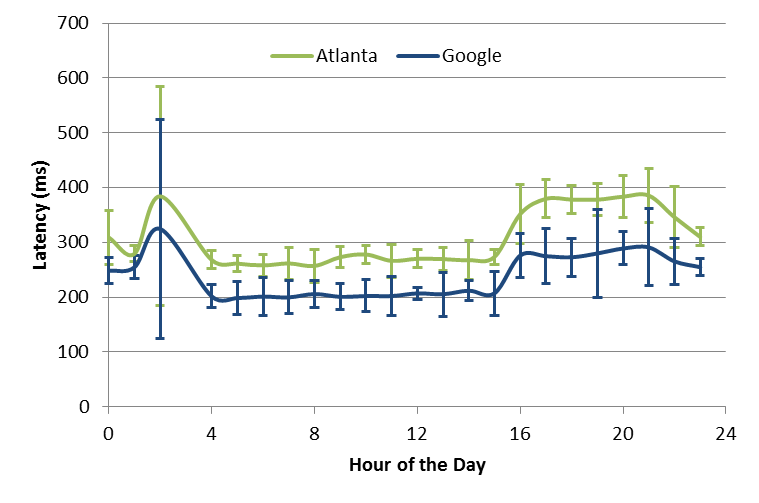
\includegraphics[height=0.2 \textheight,width=0.48 \textwidth]{14.png}
   \end {center}
 \caption{Mean latency values to the local hour of the day to the servers at Atlanta and Kansas (GOOGLE DNS). Latency to both servers (Atlanta \& Kansas) is high (more than 300ms) and become more inconstant throughout peak hours.}\label{Fig:15}
\end{figure}

\section {Discussions and Recommendations}
\indent On the basis of findings from our study, we present following takeaway points and recommendations in order to enhance broadband performance in Pakistan.
\begin{itemize}
  \item The ISPs are not fulfilling their promise of advertised rates to users in Pakistan.
  \item The regions where both land line and wireless (fixed) broadband connections are available; wireless broadband outperforms land line.
  \item Throughput is not only limiting factor in broadband performance; latency values to international servers also affect broadband performance.
\end{itemize}
\indent Keeping these insights in perspective, we provide following strategy recommendations for Pakistan.\\
\subsection {Beneficial for customers, ISPs and regulating authorities}
\indent From our continuous routers data set, it is evident that most of the customers do not achieve rates that are advertised to them by their ISPs. The regulating authorities are required to develop frameworks that result in continuous monitoring of broadband services to home users in Pakistan. We provide methods to develop such a framework. Our method will help regulators to draft regulating policies continuously and will help customers and ISPs to be enlightened in terms of services. Thus, we recommend ways and approaches for continuous measurement of broadband connections in Pakistan that will help customers, ISPs and regulators to take informed decisions.
\subsection {Private investment in local infrastructure}
 \indent Regulators should assist in aiding private investment in local infrastructure. Our findings suggest that throughput is not only cause for performance degradation in Pakistan. Latency to international servers and services also affect user's experience particular to well-known and popular websites. Thus authorities, in spite of increasing throughput rate in the country should provide maximum incentive to private investors to invest in local infrastructure in or near Pakistan. Authorities should also provide favorable environment for peering between different ISPs so that content can be fetched quickly. Whichever of these, will result in reduction of latency values. Reducing distance to international Internet content for consumers in Pakistan will definitely enhance users experience. Regulators should create environment that private investors may invest in following categories in order to decrease latency values.
 \subsection {Creating favorable environment for native versions of prevalent services}
\indent  Pakistan already has some local versions of international services that are popular like olx.com.pk,  google.com.pk, travian.com.pk. The state can help create a favorable environment in order to improve local versions of international services. This can considerably improve performance of broadband connections in Pakistan.
\subsection {Reducing distance to content by creating local data centers}
\indent Authorities should make efforts and provide incentives to private investors in order to create local data centers for users in Pakistan. State cooperation with popular service providers to build up data centers that are geographically closer to Pakistan should be encouraged. This will help enhance performance for popular services in Pakistan.
\subsection {Peering between ISPs:}
 \indent Authorities and private entities should make an effort in order to create multiple exchange points between different ISPs. This will result in traffic exchange locally .For example, in case of route to New Delhi, it was traversed via Singapore. If local exchange point is created between ISPs, it will make performance of broadband connection better in Pakistan and India, both.

\section {CONCLUSION}
We have presented results of our study for fixed landline and wireless broadband performance in Pakistan. Our results indicate that (a) ISPs are not fulfilling the promise of advertised rates to users (b) Wireless broadband outperforms fixed land line where both are available (c) Throughput is not the only reason for degradation in broadband performance, latency to prevalent websites and services also plays a vital role in performance deprivation (as defined in terms of geographic distance and ISP peering). Thus, many encouraging Internet aspects guaranteed by ISPs are not recognized in Pakistan and a number of problems associated with latency and throughput degrade broadband performance.\\
\indent We advise regulators to implement continuous monitoring of broadband Internet service providers either by using router based or host based measurement methods at a number of locations and service plans. Initiatives should also be taken for investment in local infrastructure to bring international content and services closer to the country users.According to BCG e-friction index model ~\cite{31} Pakistan lies at the top with high e-friction score of 82, topping mostly all the countries except Nigeria. High e-friction countries are in great risk of missing out on a high-impact stimulant of growth and job creation. We hope that our contribution in benchmarking ISPs of Pakistan will benefit end customers and help regulators to make informed decisions. It will also provide insights to regulators draft new broadband performance policy for Pakistan.\\
\indent In future work, we plan to benchmark mobile cellular services on achieved data rates. Pakistan is on verge of launching 3G and 4G services ~\cite {32,33}.  Thus, a performance comparison of fixed broadband with mobile broadband would be interesting and meaningful.




%\begin{figure}[h!]
%\begin {center}
   %Requires \usepackage{graphicx}
 %  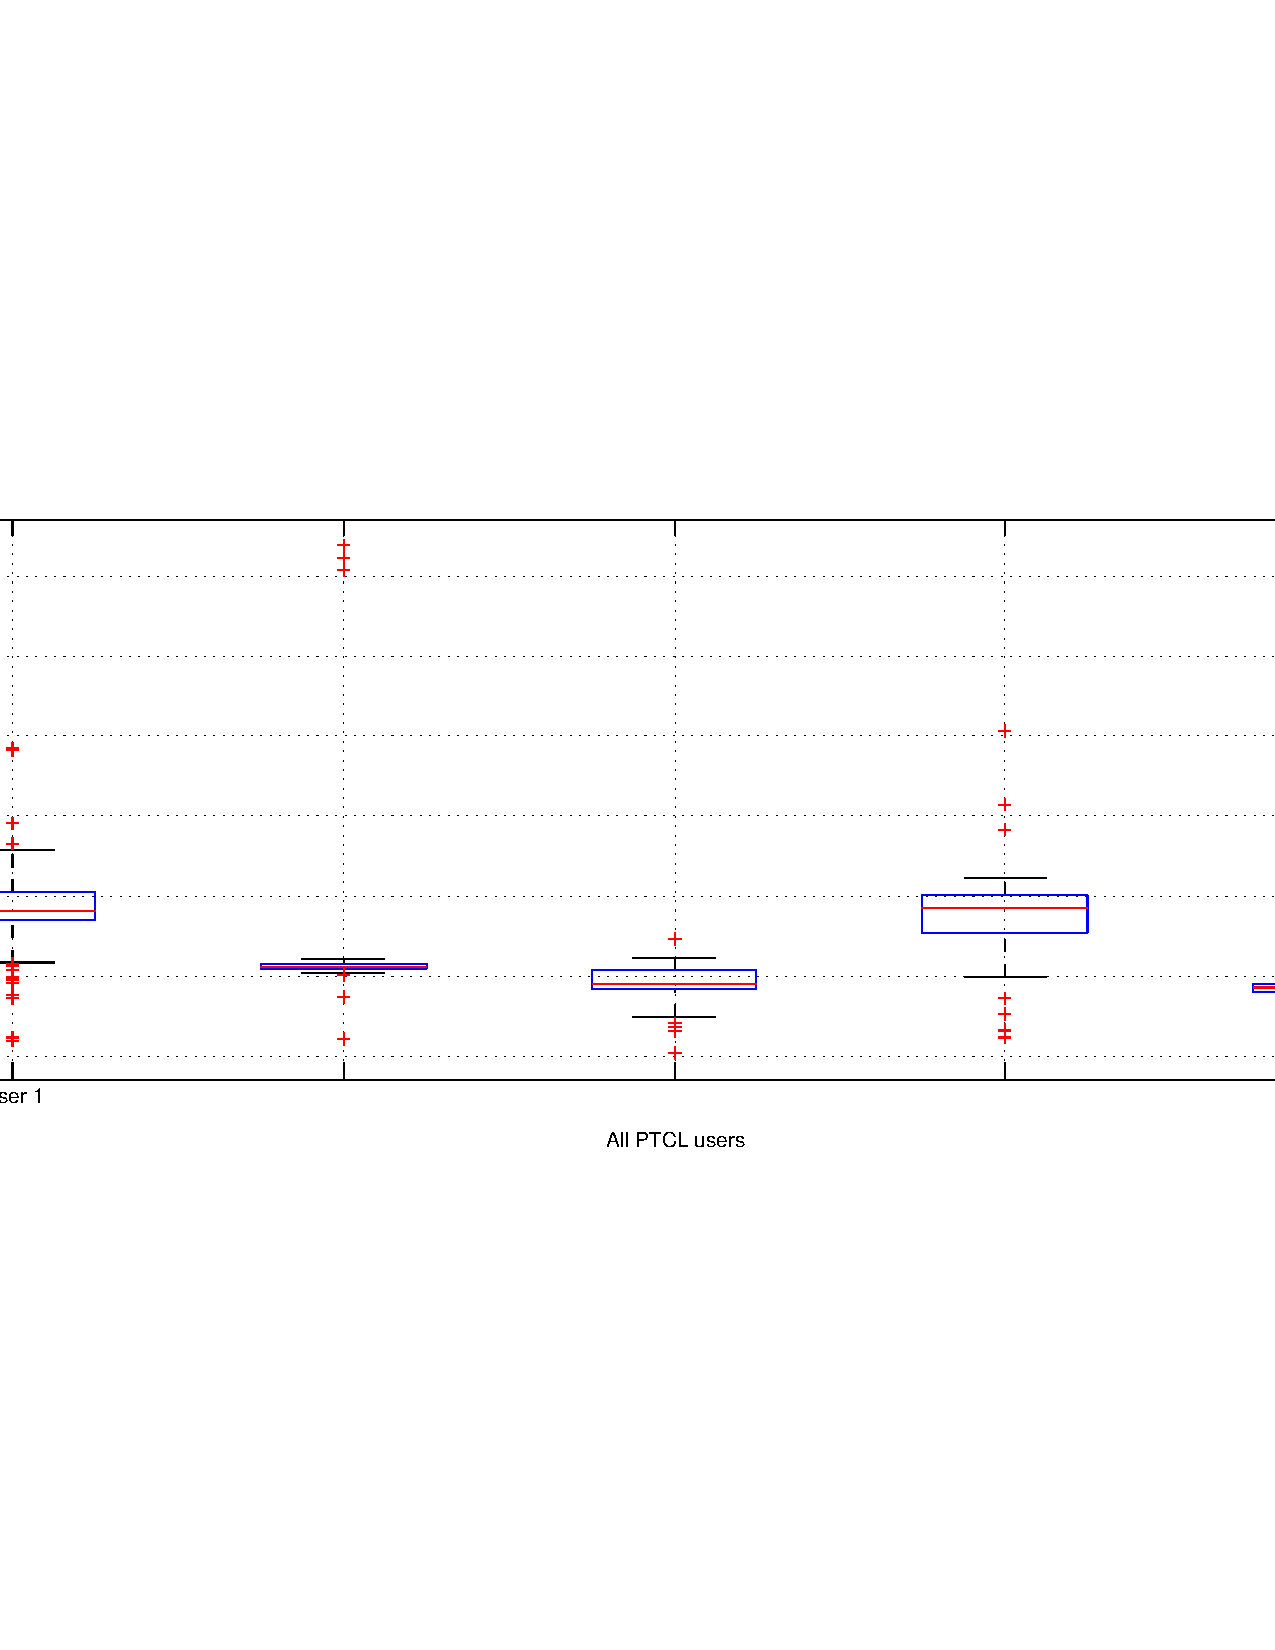
\includegraphics[height=0.2 \textheight,width=0.4 \textwidth]{16.png}
  % \end {center}
 %\caption{\textbf{BCG e-index score 2013}}
%\end{figure}




\begin{small}

\bibliographystyle{IEEEtran}
\balance \bibliography{new1}
\end{small}
\end{sloppypar}
\end{document}
\endinput


%%%%%%%%%%%%%%%%%%%%%%%%%%%%%%%%%%
% : vim: set spelllang=en_us spell ts=4 shiftwidth=4 foldmethod=indent autoindent ignorecase : %
